
\subsection{Event Selection}
\label{sec:resolved_selection}
The final state of interest consists of one charged lepton, one neutrino, 
and four quarks, two of which are b-quarks. Hence the detector signature
consists of one  charged lepton ($e$/$\mu$), large $\met$, and four or more
anti-$k_t$ jets of which two are $b$ jets from the $h$ decay while the other
two are light jets from the hadronic decay of the $W$ boson. One challenge
in the event reconstruction is to correctly identify the pair of light jets
from the $W$ boson decay. This information is also used to solve the $z$
component of the neutrino momentum. For the HH signal there is an additional
complication due to the fact that one of the 
$W$ bosons is off-shell, and thus for this $W$ there is no $W$ mass constraint. 
This section details the stages of the event reconstruction and the
progression towards the final selection which defines the signal
region.  In addition, signal depleted control regions are defined in the
next section which are used to check the consistency of the SM background
predictions with the data in the control regions. The search
has been kept ``blinded'' until the comparison between data and
simulation of backgrounds are well understood in the signal depleted
control regions.

\subsection{Trigger requirement}

Events are selected using the unprescaled single lepton triggers. The list of triggers used in 
this analysis is shown in Table~\ref{tab:triggers}. Events are selected with a logical OR between 
the triggers listed in Table~\ref{tab:triggers}.

\begin{table}[htbp!]
\begin{center}
 \begin{tabular}{|c|c|}
  \hline
  Dataset & Trigger items \\
  \hline
  \multirow{2}{*}{2015} & mu20\_iloose\_L1MU15  \\
    & mu50  \\
    & e24\_lhmedium\_L1EM18VH (MC)  \\
    & e24\_lhmedium\_L1EM20VH (data)  \\
    & e60\_lhmedium  \\
    & e120\_lhloose  \\
  \hline
  \multirow{8}{*}{2016 - Period A} & mu24\_iloose\_L1MU15 (MC)  \\
    & mu24\_iloose (data)  \\
    & mu40  \\
    & e26\_lhtight\_nod0\_ivarloose  \\
    & e60\_lhmedium\_nod0  \\
    & e60\_medium  \\
    & e140\_lhloose\_nod0  \\
    & e300\_etcut  \\
  \hline
  \multirow{7}{*}{2016 - Period B-D3} & mu24\_ivarmedium  \\
    & mu50  \\
    & e26\_lhtight\_nod0\_ivarloose  \\
    & e60\_lhmedium\_nod0  \\
    & e60\_lhmedium  \\
    & e140\_lhloose\_nod0  \\
    & e300\_etcut  \\
  \hline
  \multirow{7}{*}{2016 - Period D4-E3} & mu26\_ivarmedium  \\
   & mu50  \\
   & e26\_lhtight\_nod0\_ivarloose  \\
   & e60\_lhmedium\_nod0  \\
   & e60\_lhmedium \\
   & e140\_lhloose\_nod0  \\
   & e300\_etcut  \\
  \hline
  \multirow{7}{*}{2016 - Period $\ge$ F} & mu26\_ivarmedium   \\
   & mu50  \\
   & e26\_lhtight\_nod0\_ivarloose  \\
   & e60\_lhmedium\_nod0  \\
   & e60\_lhmedium  \\
   & e140\_lhloose\_nod0  \\
   & e300\_etcut  \\
  \hline
 \end{tabular}
\end{center}
\caption[List of triggers used]{Summary of trigger items used for 2015 and 2016 data. For 2016 data, different triggers were used for different data run periods. 
All triggers are unprescaled.}
\label{tab:triggers}
\end{table}


\subsubsection{Pre-selection}
The following selection criteria are applied at the pre-selection level to the recorded events:
\begin{itemize}
\item Good detector conditions are required based on data quality assessment. See Appendix ~\ref{app:app-data} for more details.
  \iffalse
  \footnote { {\small
\begin{verbatim}
  eventInfo->errorState(xAOD::EventInfo::EventFlagSubDet::Tile) == xAOD::EventInfo::Error,
  eventInfo->errorState(xAOD::EventInfo::EventFlagSubDet::LAr)  == xAOD::EventInfo::Error,
  eventInfo->errorState(xAOD::EventInfo::EventFlagSubDet::SCT)  == xAOD::EventInfo::Error, 
  (eventInfo->eventFlags(EventInfo::Core) \& 0x40000) is true.
\end{verbatim}
}
}
\fi

\item The presence of a  primary vertex with at least two
  tracks. Among all primary vertices, that with the highest
	$\sum p_{{\rm T,trk}}^{2}$, where
	$p_{{\rm T,trk}}$ is the transverse momentum of tracks
	associated with the vertex, is retained as the primary
  interaction vertex;
\item at least one SignalElectron ($e$) or SignalMuon ($\mu$), as defined in Section~\ref{sec:el_reco} and Section~\ref{sec:mu_reco}, and it must be trigger matched to the 
corresponding HLT object which fires the trigger;
\item at least four jets, of which two and only two are $b$-tagged.
\end{itemize}

\subsection{Event Reconstruction}
\label{ssec:event_reco_res} 
%%The final state of our signal consists of one charged lepton, one neutrino, and four quarks, 
%%two being $b$-quraks. Hence the detector signature consists of one charged lepton, missing 
%%transverse momentum, and four or more jets of which two are $b$ jets from the $h$ decay while 
%%the other two are light jets from the hadronic decay of the $W$ boson. 
Events are reconstructed by first requiring exactly two 2 $b$-tag jets and at least two light
jets and at most three light jets. In events with three light jets, the pair with the 
lowest $\Delta R$ between them are selected as $W$ jet candidates. This
procedure yields the correct jet assignment in 70\% of the cases for
signal events where the
hadronic daughters of the $W$ boson can be correctly matched to reconstructed
jets. %as described in Appendix~\ref{app:jetTruthStudies}.
%After preselection both light jets from $W$ bosons can be correctly matched in  20 \% of events.(see Appendix \ref{sec:BenStudy}).  

The event kinematics of the $H \to WW^* \to l \nu qq$ topology can be fully
reconstructed. In fact, among all four-momenta of the final state particle,
only the component of the neutrino momentum along the beam axis, $p_z$ in the following, is unknown while its transverse
momentum is the measured $\met$. Imposing the relation:
\begin{equation}
\label{eq:mh1}
m_h^2 = (p^l + p^{\nu} + p^{j1} + p^{j2})^2
\end{equation}
where $p^i$ is the four-momenta of particle $i$, the neutrino $p_z$ can be
reconstructed using the relations:
\[
p_E^{\nu} = E^{\nu} = \sqrt{P_T^2 + p_z^2} \quad p_x^{\nu} = P_Tcos(\phi) \quad p_y^{\nu} = P_T sin(\phi)
\]
where $\phi$ is the azimuthal angle of the $\met$, $E^{\nu}$ the neutrino
energy, $p_x$ and $p_y$ the two transverse spatial components of the neutrino momentum.
Equation \ref{eq:mh1} is a quadratic expression in $p_z$. It can have two real,
one real  or two complex solutions. In the last case only the real part of the
complex solution is taken into account, therefore a single value of $p_z$ is
obtained. In the first case the solution with the neutrino direction closest
to the charged lepton is retained. It has been shown that this algorithm
selects the correct solution in approximately 60\% of the cases
(see Appendix~\ref{app:nupz_studies}).
\newpage
\subsection{$\mathbf{bb\tau\tau}$ analysis overlap removal}
In order to remove overlap with the $bb\tau \tau$ analysis we reject
any event containing at least one hadronic $\tau$ candidate that could be
identified by the $bb\tau\tau$ analysis, that fullfill the following
requirements:
\begin{itemize}
\item $p_T > 20$ GeV and $|\eta| < 2.5$;
\item one or three prongs;
\item unit charge;
\item pass the medium $\tau$ ID BDT working point.
\end{itemize}

The rejection of such events causes a signal efficiency drop of about 3\%.

\subsection{Kinematic selection}
\label{subsec:kincuts}


Kinematic selection is used to suppress mainly $t\bar{t}$ background while keeping
high signal efficiency.  A schematic view of the $HH \to WW{*}b\overline{b}$ and the
$t \bar{t} \to WWbb$ event topology is shown in Figure ~\ref{fig:cartoon}.

\begin{figure}[h]
\begin{center}
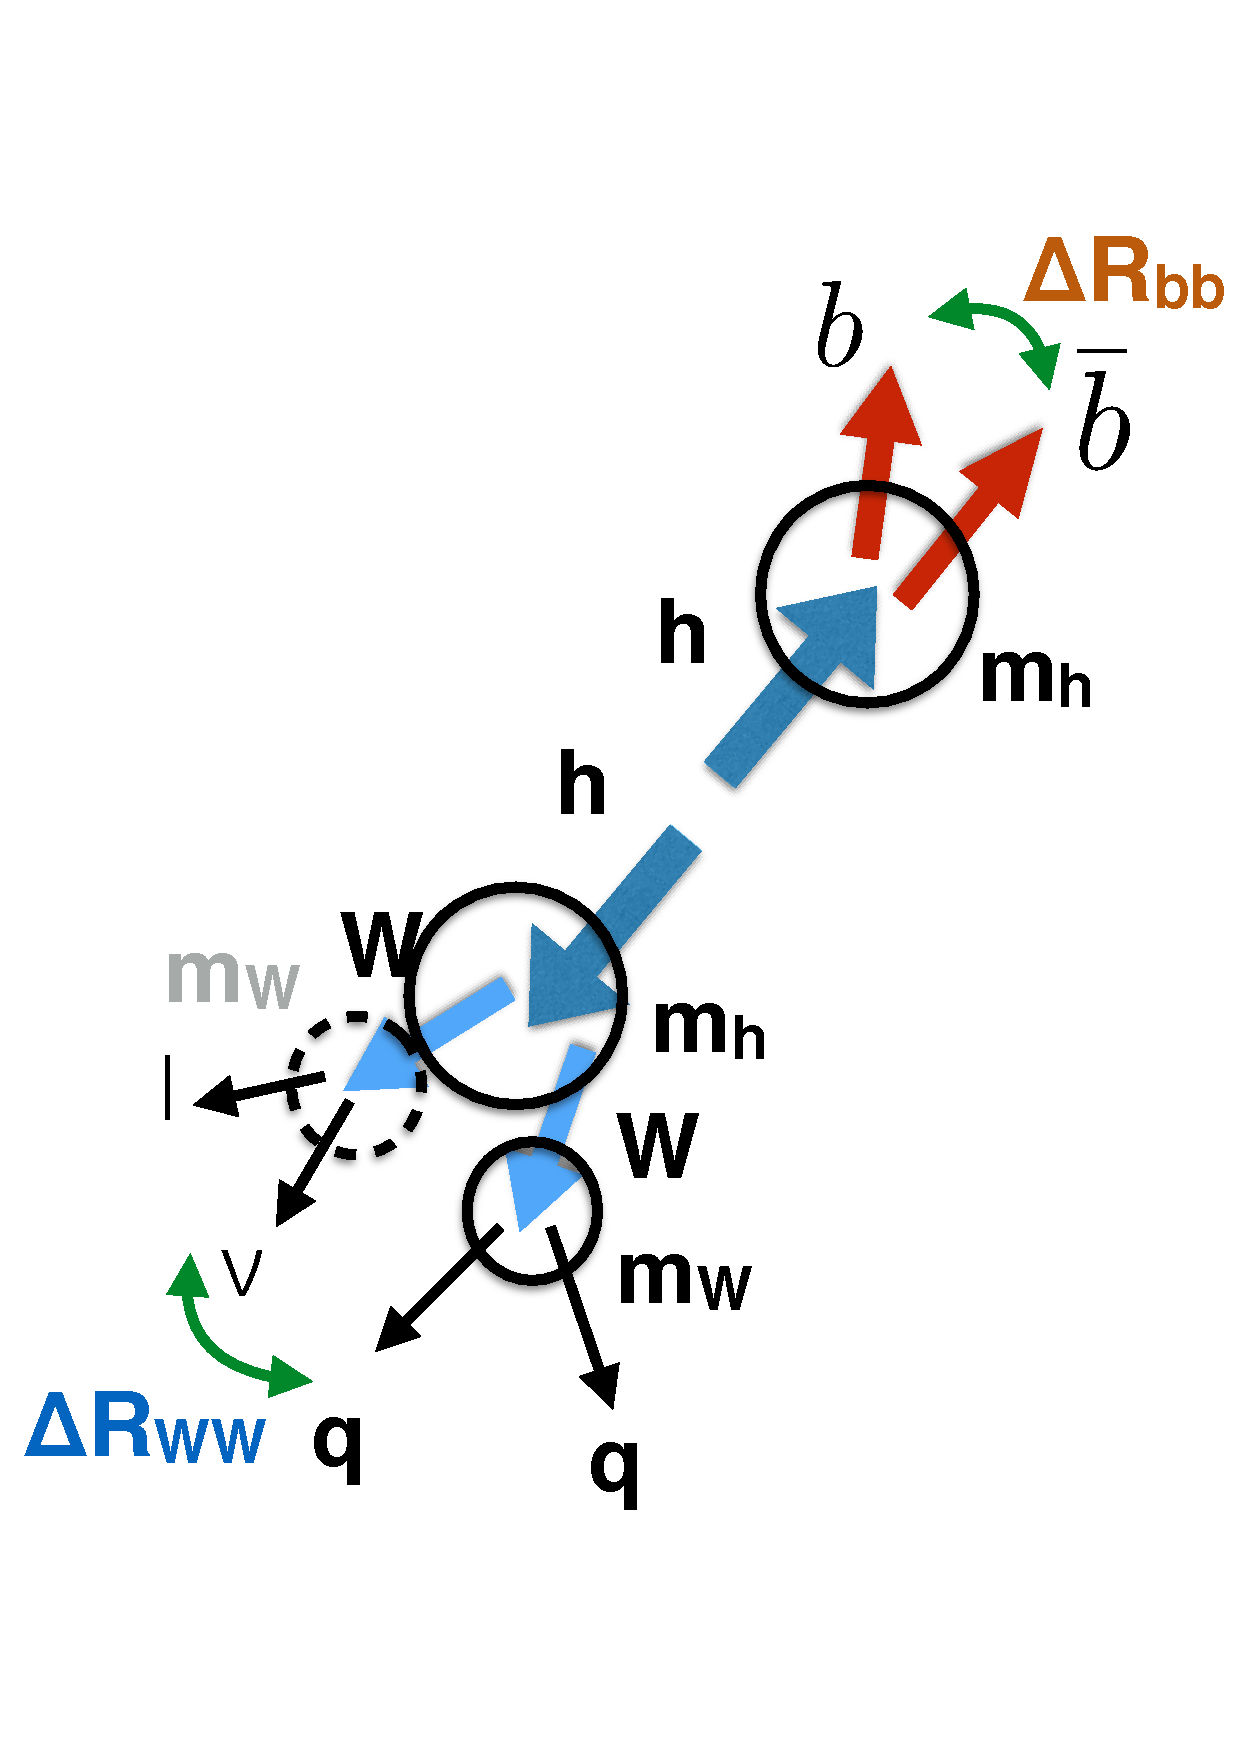
\includegraphics[width=0.45\textwidth]{figures/cartoon_hh.pdf}
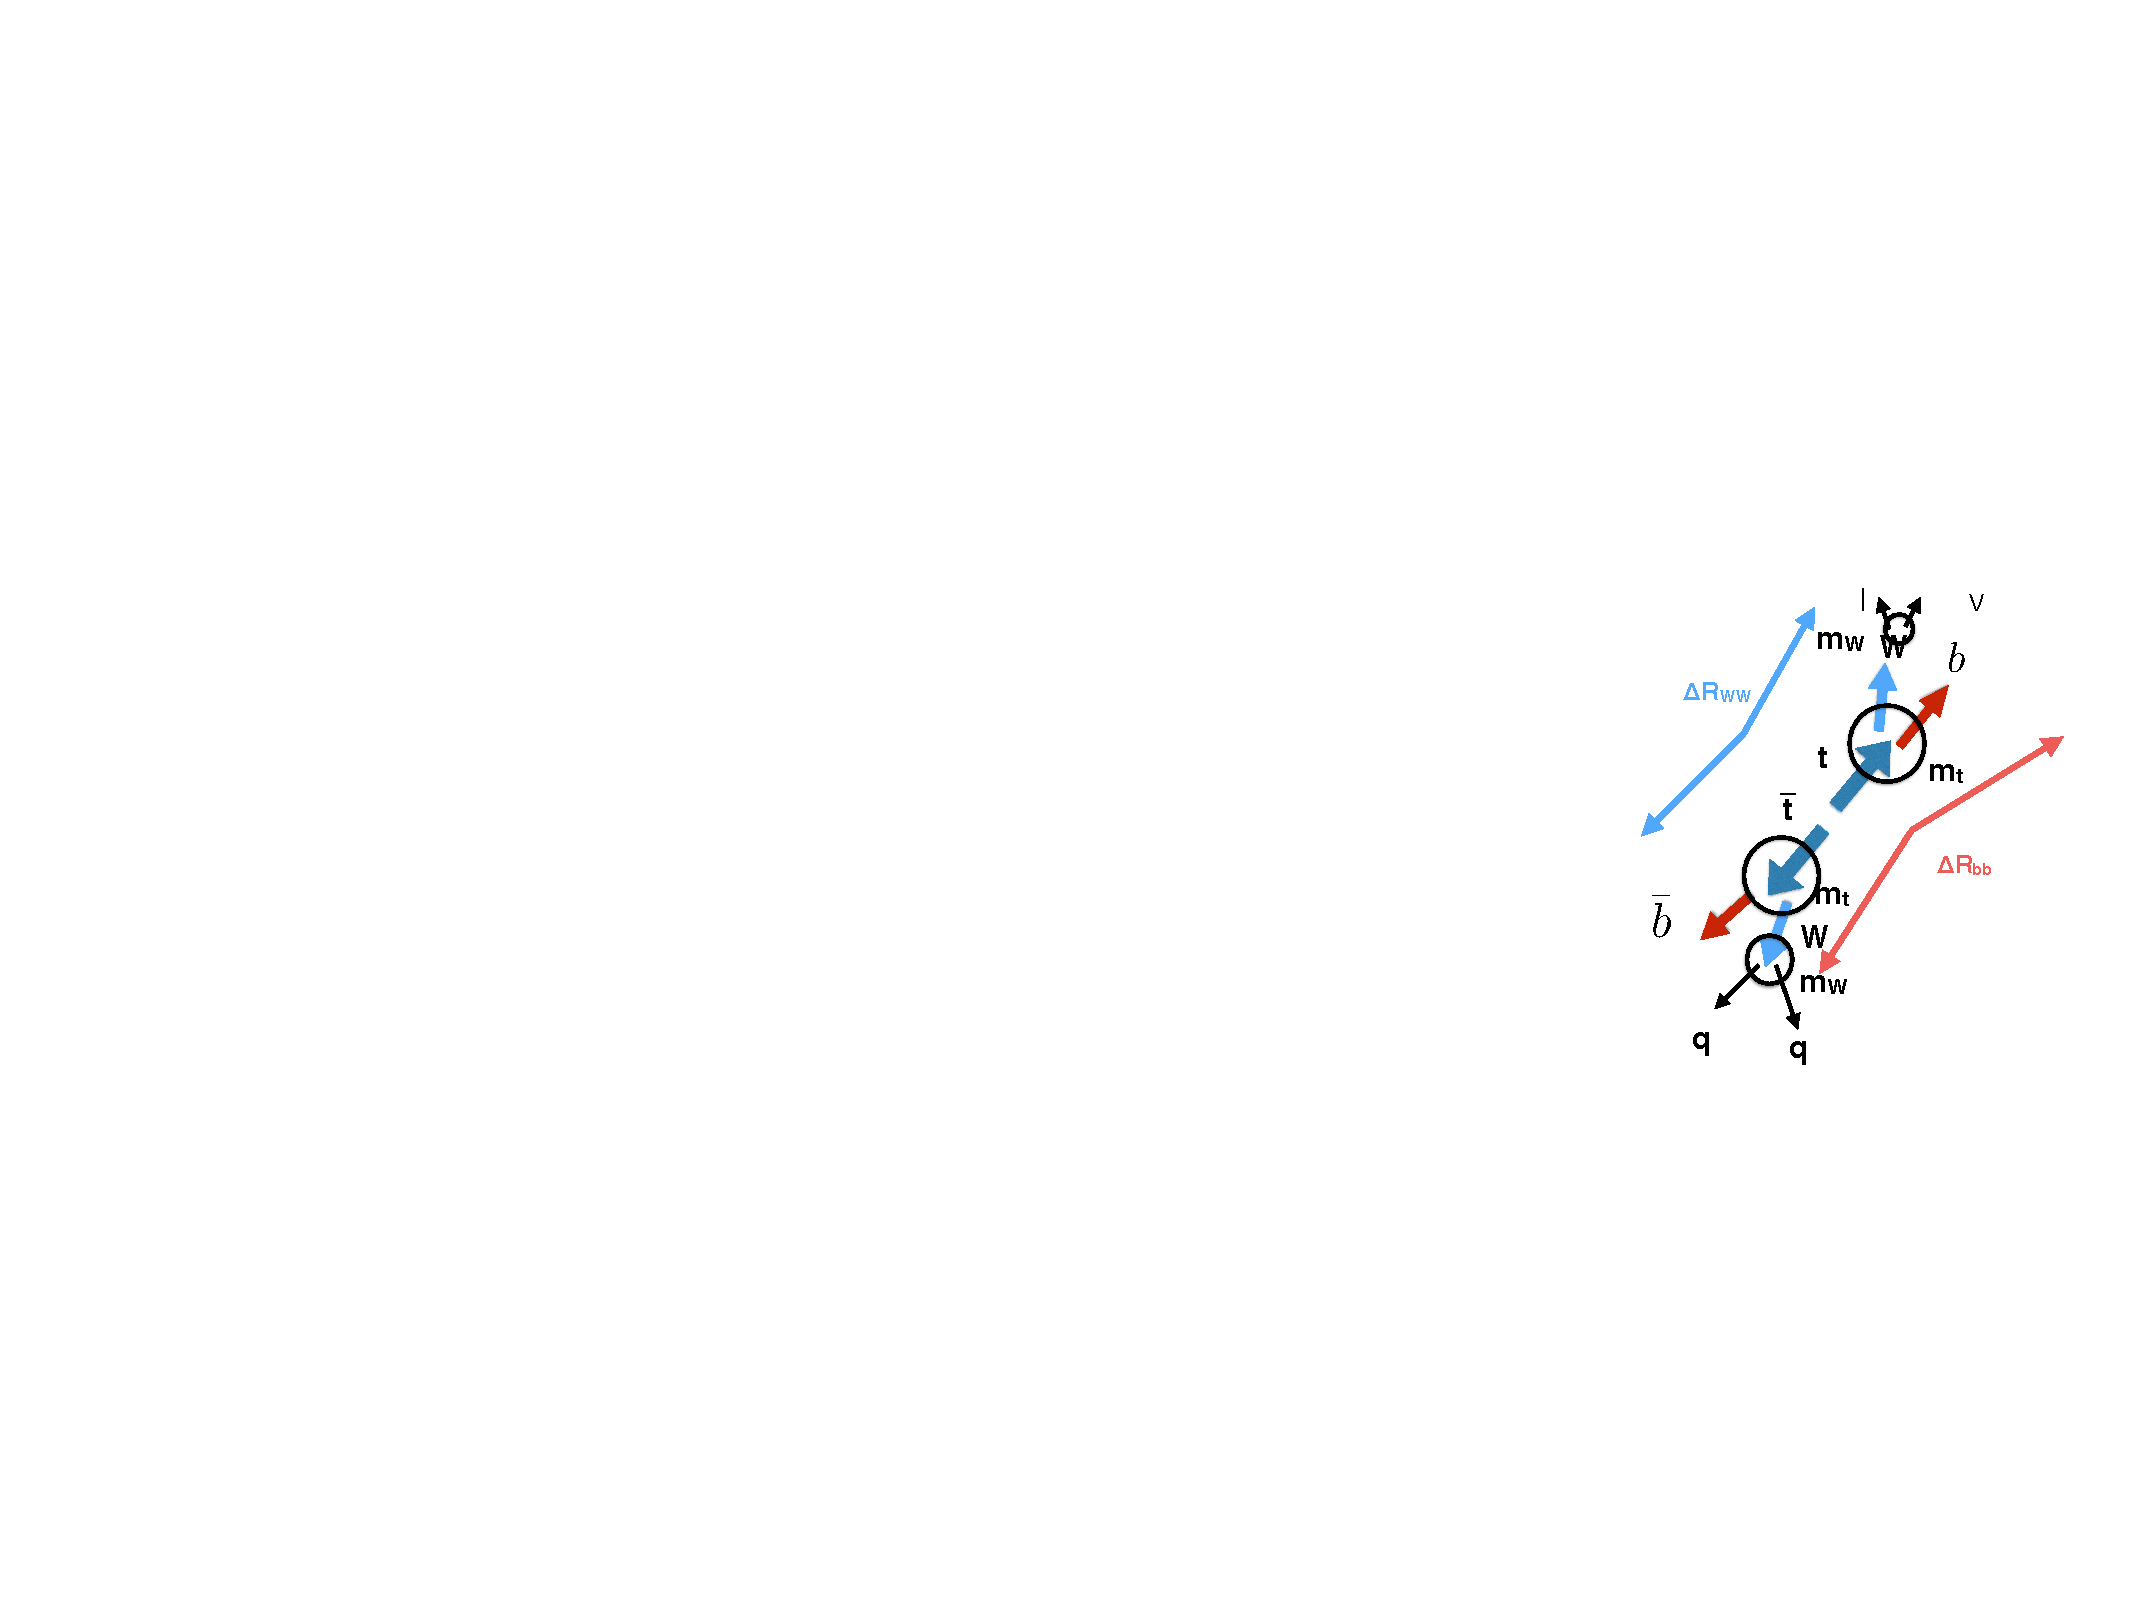
\includegraphics[width=0.45\textwidth]{figures/cartoon_tt.pdf}
\caption[Comparison signal and \ttbar events]{Schematic view of a $HH \to WWbb$ event compared to a $t\bar{t} \to WWbb$ event.} 
\label{fig:cartoon}
\end{center}
\end{figure}

The $t \bar{t}$ events are typically characterized by two $b$-jets and
two $W$ bosons such that the $\Delta R$ separation between the two
$b$-jets and between the $W$ bosons is large. On the contrary, in particular
when the invariant mass of the $m_{HH}$ is high, the signal is characterized
by two $b$-jets which are close together in $\Delta R$ and by two $W$ bosons
which are also relatively closer than in the $t \bar{t}$
case. Moreover, while for the signal the two $b$-jets have an
invariant mass equal to $m_h$, this is not necessarily the case for the $t \bar{t}$ background.  Following these considerations, the typical separation variables are: 
\begin{itemize}
\item the $p_T$ of the $b \bar{b}$ pair ($p_T^{bb}$);
\item the $\Delta R$ of the $b \bar{b}$ pair ($\Delta R^{bb}$);
\item the $p_T$ of the $WW$ pair ($p_T^{WW}$);
\item the $\Delta R$ of the $WW$ pair ($\Delta R^{WW}$);
\item the mass of the $WW$ system computed using the calculated neutrino
      longitudinal momentum ($m_{\rm WW}$). This value is exactly equal to $m_h$
      if a real solution is found, it is larger if no real solution is found;
\item the invariant mass of the di-Higgs boson candidate system ($m_{HH}$). 
\item the invariant mass of the 2 b-jets boson system ($m_{bb}$). 

\end{itemize}


\subsection{Signal region definitions}
\label{subsec:SR}
The signal selection criteria have been optimized by maximizing the Poisson significance at the end of the selection based on MC simulation \footnote{a two step procedure has been implemented. In the first step each selection criteria is optimized, in the second step, all selections are set to their optimal value and selections are varied one by one to
look for a different optimization point. Correlation among variables could in fact spoil the results obtained at the first step.}. The Poisson significance formula depends on the absolute yield of expected signal and
background events. For the optimization formula the \ttbar background was
normalized to data with $m_{bb} < 100$ GeV or $m_{bb} > 140$ GeV, where the majority of the signal is rejected. Four signal
hypotheses have been used in the optimization:
\begin{itemize}
\item{ a heavy Higgs with $m_S = 500$ GeV and $m_S = 700$ GeV (defined as low-mass analysis)},
\item{ a heavy Higgs with $m_S = 2000$ GeV (defined as high-mass analysis) and}
\item{ a non-resonant di-Higgs production (defined as non-resonant analysis).}
\end{itemize}
An additional mass point with $m_S = 1400$ GeV was also checked. The resulting selection and the corresponding sensitivity are very similar to the selection for $m_S = 2000$ GeV, and hence that selection is dropped.{\footnote {See \url {https://indico.cern.ch/event/641988/contributions/2604588/attachments/1465307/2265002/bbWW_Weekly_Optimization_Revisited_24May2018.pdf}}} 
%The signals have been normalized to the Run 1 upper limit scaled by the $13/8$ TeV cross section ratio expected from the
%PDF luminosity scale of a narrow resonance of that mass. 

The signal regions for the  reference signal hypotheses are summarized in 
Table~\ref{tab:sig_reg_summary}.


\begin{table}
\begin{center}
\begin{tabular}{c|c|c|c|c}
 variable & \emph{Non-Res} & \emph{m500} & \emph{low-mass} & \emph{high-mass}\\
\hline
$\met$ (GeV)		&$> 25$&$>25$&$> 25$& $> 25$ \\
$m_{WW}$ (GeV) 	   		&$< 130$ &$< 130$ & $< 130$& no-cut\\
$p_{\rm T}^{bb}$ (GeV) 		&$> 300$& $> 210$&$> 210$&$> 350$\\
$p_{\rm T}^{WW}$ (GeV) 		&$> 250$&$> 150$&$> 250$&$> 250$ \\
$\Delta R_{WW}$  		&no-cut& no-cut&no-cut&$<1.5$\\
$m_{bb}$ (GeV)   		&105-135&105-135&105-135&105-135\\
\end{tabular}
\caption[Criteria for \emph{non-res}, \emph{m500}, \emph{low-mass} and 
    \emph{high-mass} selection]{Criteria for non-resonant, \emph{m500}, \emph{low-mass} and 
    \emph{high-mass} selection. The $m_{HH}$ window is not applied for 
    non-resonant signal, and for resonant signals $m_{HH}$ depends on 
    the mass.} 
\label{tab:sig_reg_summary}
\end{center}
\end{table}


The \emph{non-res} and \emph{m500} selections are exclusively used for non-resonant signal and resonant signal with mass 500 GeV respectively. The \emph{low-mass} selection is used for signal masses from 600 to 1300 GeV, while the \emph{high-mass} selection is used for signals with masses between 1400 and 3000 GeV. In addition, requirements are placed on the reconstructed di-Higgs invariant mass ${m_{HH}}$ as a function of the signal resonance mass ${m_{S}}$, as shown in Table \ref{tab:mhh_sig_cuts}. The resolution of the reconstructed $m_{HH}$ ranges from 6\% at 500 GeV to 10\% at 3000 GeV.

\begin{table}
\begin{center}
\begin{tabular}{c|c|c|c|c|c}
$m_{S}$ (GeV)      &   500   &   600   &   700   &   750   &   800 \\
$m_{HH}$  (GeV) & 480-530 & 560-640 & 625-775 & 660-840 & 695 - 905 \\ 
\hline 
$m_{S}$ (GeV)      &  900   &   1000  	   &  1100   	&  1200   		&   1300    \\
$m_{HH}$  (GeV) & 760-970	& 840-1160 & 925-1275	&1010-1390	&1095-1505  \\
\hline 
$m_{S}$ (GeV)      &   1400  		&  1500   		&  1600   		& 1800  		& 2000\\
$m_{HH}$  (GeV) &1250-1550	&1340-1660	&1430-1770	& 1750-2020 	& 1910-2170\\
\hline

\hline 
$m_{S}$ (GeV)      &   2250  		&  2500   		&  2750   		& 3000  		& \\
$m_{HH}$  (GeV) &2040-2460	&2330-2740	&2570-2950	& 2760-3210 	& \\
\end{tabular}
\caption[Window selection on ${m_HH}$]{Window selection on $m_{HH}$ as a function of the resonance mass
  $m_{S}$.}
\label{tab:mhh_sig_cuts}
\end{center}
\end{table}


\subsection{Background Determination}
In the present analysis we expect that at the end of the event selection the
sample will be largely dominated by $t \bar{t}$ and multi-jet background, therefore the $t\bar{t}$ background normalization
is derived from data while, as described in Sec. \ref{sec:multijet}, the multi-jet
background is derived using a data-driven ABCD method.
For all the other backgrounds, e.g. di-boson, Higgs, $W$+jets, the
MC is used appropriately normalized by using the expected cross sections and the
integrated luminosity that has been collected.

\subsubsection{Top normalization and control region}
\label{subsec:topCR}
The \ttbar background is normalized and validated using  dedicated
control regions (CR). Three CR's are defined, one for the SR's of the \emph{non-res} (CR1), one for the \emph{low-mass} analysis (CR2), and one for the \emph{high-mass} analysis (CR3).  The CRs are defined in Table \ref{tab:CRdef}.


Table \ref{tab:CR1} through \ref{tab:CR3} show the number of observed
events and expected background events in the top CRs, and also in the sideband across selections that serve as validation regions. The final signal region is defined by $m_{bb}$ of $105~\textrm{GeV} < m_{bb} < 135~\textrm{GeV}$ based on optimization. The sidebands are orthogonal to the SR by virtue of having the $m_{bb}$ reversed. $m_{bb} < 100$ GeV or $m_{bb} > 140$ GeV defines the sidebands in which the control regions are defined.  The 5 GeV buffer region is kept on both sides so as to be less affected by systematic effects at the edge. Fig.~\ref{fig:mbb_signal} shows $m_{bb}$ for various signal mass points. A comparative study of signal over background in these three regions shows that S/B in the final SR is 5 (20) times higher than in the sidebands for m2000 (non-resonance) while S/B in the final SR is approximate twice as high as in the buffer zones.  Table~\ref{tab:sigOverBkg} shows the ratios of S/B in the buffer zones and sidebands compared to the S/B in the final SR. \newline

\begin{figure}[!h]
\begin{center}
\includegraphics*[width=0.9\textwidth] {figures/bbMass_X500_X700_X1400_X2000_X3000.eps}
\caption[$m_{bb}$ resolution for signal and sum of backgrounds.]{$m_{bb}$ resolution for signal samples.}
\label{fig:mbb_signal}
\end{center}
\end{figure}

\begin{table}
\begin{center}
\begin{tabular}{c|c|c|c|c}
Selection & non-res & m500 & m700 & m2000\\
\hline
Buffer/SR              	& 1.85 & 1.95  & 1.90 & 1.63\\
\hline
 Sidebands/SR	       & 20.5 & 12.6 & 13.4 & 5.6\\
\hline 
\end{tabular}
\caption[S/B ratios]{The ratios of S/B in the buffer zone and sidebands compared to the S/B in the final SR. } 
\label{tab:sigOverBkg}
\end{center}
\end{table}

%%%%%%%%%%%%%%
\begin{table}
\begin{center}
\begin{tabular}{c|c|c|c}
 variable 						&CR1 				& CR2 	& CR3 \\
\hline					
$m_{bb}$ (GeV)						& $m_{bb} < 100$ or $m_{bb} > 140$ & $m_{bb} < 100$ or $m_{bb} > 140$ & $m_{bb} < 100$ or $m_{bb} > 140$\\
$m_{WW}$ (GeV)   				& $<130$ 		 		& $<130$		& no-cut \\
$p_{\rm T}^{bb}$ (GeV) 			& $>300$ 		 		& $>210$		&$>350$\\
\hline


\end{tabular}
\caption[Definition of the kinematic regions used to normalize the Top background]{Definition of the kinematic regions used to normalize the Top background. $m_{bb} < 100$~GeV or $m_{bb} > 140~GeV$ defines the sidebands in which the control regions are defined. Expected SM backgrounds are then checked against data at each subsequent selection.} \label{tab:CRdef}
\end{center}
\end{table}
%%%%%%%%%%%%%%%

\begin{center}
\begin{table}
\begin{tabular}{l|c|c|c|c}
\hline\hline
\multicolumn{5}{c}{\textbf{CR1}: \mbb Sideband}\\\hline\hline
Sample  	& mww 	& bbpt210 	& bbpt300 	& wwpt250 	  \\\hline
\ttbar 	& 23776.6 $\pm$ 87.2 	& 531.7 $\pm$ 13.1 	& 109.9 $\pm$ 5.9 	& 63.9 $\pm$ 4.6 \\\hline 
QCD 	& 13310.5 $\pm$ 500.3 	& 250.2 $\pm$ 30.6 	& 33.7 $\pm$ 4.1 	& 21.4 $\pm$ 2.6	\\\hline 
W+jets 	& 3938.9 $\pm$ 31.1 	& 124.7 $\pm$ 3.5 	& 29.3 $\pm$ 1.4 	& 17.1 $\pm$ 1.1 	\\\hline 
SingleTop 	& 1605.4 $\pm$ 18.0 	& 76.0 $\pm$ 3.8 	& 20.1 $\pm$ 2.0 	& 13.5 $\pm$ 1.7\\\hline 
Dibosons 	& 109.9 $\pm$ 2.7 	& 8.3 $\pm$ 0.8 	& 2.2 $\pm$ 0.4 	& 1.5 $\pm$ 0.4 	\\\hline 
Z+jets 	& 1107.6 $\pm$ 8.4 	& 27.1 $\pm$ 0.8 	& 6.7 $\pm$ 0.4 	& 2.4 $\pm$ 0.2 	\\\hline 
\hline
Background Sum 	& 43849.0$\pm$ 509.2 	& 1017.9$\pm$ 33.7 	& 201.9$\pm$ 7.6 	& 119.8$\pm$ 5.7 \\\hline 
\hline
XhhSM 	& 44.6 $\pm$ 2.2 	& 9.1 $\pm$ 0.7 	& 1.5 $\pm$ 0.2 	& 1.1 $\pm$ 0.1 	\\\hline 
Data 	& 43902.0 	& 1069.0 	& 206.0 	& 138.0 \\\hline 
\hline
\end{tabular}
\caption[The number of events in the $m_{bb}$ sideband for the non-res selection]{ The number of observed
events and expected background events in the $m_{bb}$ side-bands for
the \emph{non-res} selection. The top CR1 is defined at the bbpt300
selection. No NF has been applied to the background yields to show the level of data/expectation agreement before normalizing ttbar.  Only statistical uncertainties are shown.}
\label{tab:CR1}
\end{table}
\end{center}

\begin{center}
\begin{table}
\begin{tabular}{l|c|c|c|c}
\hline\hline
\multicolumn{5}{c}{\textbf{CR2}: \mbb Sideband}\\\hline\hline
Sample  	& mww 	& bbpt210 	& wwpt150 	& hh500  \\\hline
\ttbar 	& 23776.6 $\pm$ 87.2 	& 531.7 $\pm$ 13.1 	& 432.7 $\pm$ 11.8 	& 35.5 $\pm$ 3.2 		\\\hline 
QCD 	& 13310.5 $\pm$ 500.3 	& 250.2 $\pm$ 30.6 	& 206.3 $\pm$ 25.3 	& 16.9 $\pm$ 2.1 		\\\hline 
W+jets 	& 3938.9 $\pm$ 31.1 	& 124.7 $\pm$ 3.5 	& 105.9 $\pm$ 3.3 	& 4.9 $\pm$ 0.6 	\\\hline 
SingleTop 	& 1605.4 $\pm$ 18.0 	& 76.0 $\pm$ 3.8 	& 64.9 $\pm$ 3.5 	& 2.8 $\pm$ 0.6 	\\\hline 
Dibosons 	& 109.9 $\pm$ 2.7 	& 8.3 $\pm$ 0.8 	& 6.7 $\pm$ 0.8 	& 0.9 $\pm$ 0.2 	\\\hline 
Z+jets 	& 1107.6 $\pm$ 8.4 	& 27.1 $\pm$ 0.8 	& 19.0 $\pm$ 0.7 	& 1.5 $\pm$ 0.2 		\\\hline 
\hline
Background Sum 	& 43849.0$\pm$ 509.2 	& 1017.9$\pm$ 33.7 	& 835.5$\pm$ 28.3 	& 62.5$\pm$ 3.9	\\\hline 
\hline
Xhh500 	& 3.2 $\pm$ 0.1 	& 0.6 $\pm$ 0.1 	& 0.6 $\pm$ 0.1 	& 0.2 $\pm$ 0.1 	\\\hline 
Data 	& 43902.0 	& 1069.0 	& 898.0 	& 73.0 	\\\hline 
\end{tabular}
\caption[Events in $m_{bb}$ side band for the m500 selection]{ The number of observed
events and expected background events in the $m_{bb}$ side-bands for the low-mass selection, m500. The top CR2 is defined at the bbpt210 selection. To show how well the prediction matches data, no NF has been applied to any background. Only statistical uncertainties are shown.}
\label{tab:CR2_500}
\end{table}
\end{center}
%%%%%%%%%%%%%%%%%
\begin{center}
\begin{table}
\begin{tabular}{l|c|c|c|c}
\hline\hline
\multicolumn{5}{c}{\textbf{CR2}: \mbb Sideband}\\\hline\hline
Sample  	& mww 	& bbpt210 	& wwpt250 	& hh700   \\\hline
\ttbar 	& 23776.6 $\pm$ 87.2 	& 531.7 $\pm$ 13.1 	& 175.6 $\pm$ 7.5 	& 49.9 $\pm$ 3.9 	\\\hline 
QCD 	& 13310.5 $\pm$ 500.3 	& 250.2 $\pm$ 30.6 	& 72.4 $\pm$ 8.9 	& 28.4 $\pm$ 3.5 		\\\hline 
W+jets 	& 3938.9 $\pm$ 31.1 	& 124.7 $\pm$ 3.5 	& 45.7 $\pm$ 2.1 	& 13.7 $\pm$ 1.4 	\\\hline 
SingleTop 	& 1605.4 $\pm$ 18.0 	& 76.0 $\pm$ 3.8 	& 28.4 $\pm$ 2.4 	& 6.9 $\pm$ 1.1 		\\\hline 
Diboson 	& 109.9 $\pm$ 2.7 	& 8.3 $\pm$ 0.8 	& 2.8 $\pm$ 0.5 	& 0.7 $\pm$ 0.2 		\\\hline 
Z+jets 	& 1107.6 $\pm$ 8.4 	& 27.1 $\pm$ 0.8 	& 5.8 $\pm$ 0.4 	& 2.0 $\pm$ 0.3 		\\\hline 
\hline
Background Sum 	& 43849.0$\pm$ 509.2 	& 1017.9$\pm$ 33.7 	& 330.7$\pm$ 12.1 	& 101.5$\pm$ 5.5 	\\\hline 
\hline
Xhh700 	& 4.2 $\pm$ 0.2 	& 2.2 $\pm$ 0.1 	& 1.5 $\pm$ 0.1 	& 1.0 $\pm$ 0.1 	\\\hline 
Data 	& 43902.0 	& 1069.0 	& 367.0 	& 124.0	\\\hline 


\end{tabular}
\caption[Events in $m_{bb}$ side band for the m700 selection]{ The number of observed
events and expected background events in the $m_{bb}$ side-bands for the low-mass selection, m700. The top CR2 is defined at the bbpt210 selection. To show how well the prediction matches data, no NF has been applied to any background. Only statistical uncertainties are shown.}
\label{tab:CR2_700}
\end{table}
\end{center}
%%%%%%%%%%%%%%%%%%%
\begin{center}
\begin{table}
\begin{center}
\begin{tabular}{l|c|c|c|c}
\hline\hline
\multicolumn{5}{c}{\textbf{CR3}: \mbb Sideband}\\\hline\hline
Sample  	& bbpt350 	& wwpt250 	& drww15 	& hh2000 	\\\hline
\ttbar 	& 8568.7 $\pm$ 52.1 	& 7095.6 $\pm$ 47.5 	& 1940.5 $\pm$ 25.1 	& 122.3 $\pm$ 6.5 \\\hline 
QCD 	& 1538.7 $\pm$ 252.7 	& 1359.5 $\pm$ 75.9 	& 392.7 $\pm$ 21.9 	& 20.7 $\pm$ 1.2 	\\\hline 
W+jets 	& 2259.5 $\pm$ 7.9 	& 1952.1 $\pm$ 7.4 	& 696.6 $\pm$ 4.6 	& 55.5 $\pm$ 1.1 	\\\hline 
SingleTop 	& 1778.1 $\pm$ 19.4 	& 1601.6 $\pm$ 18.4 	& 405.4 $\pm$ 9.2 	& 29.6 $\pm$ 2.6 	\\\hline 
Dibosons 	& 170.6 $\pm$ 3.9 	& 147.1 $\pm$ 3.7 	& 46.8 $\pm$ 2.1 	& 3.4 $\pm$ 0.6 	\\\hline 
Z+jets 	& 403.6 $\pm$ 2.1 	& 307.6 $\pm$ 1.8 	& 95.6 $\pm$ 1.1 	& 7.5 $\pm$ 0.3 	\\\hline 
\hline
Background Sum 	& 14719.1$\pm$ 258.9 	& 12463.5$\pm$ 91.8 	& 3577.5$\pm$ 35.0 	& 238.9$\pm$ 7.2	\\\hline 
\hline
Xhh2000 	& 25.7 $\pm$ 0.4 	& 24.0 $\pm$ 0.4 	& 9.6 $\pm$ 0.3 	& 2.9 $\pm$ 0.1	\\\hline 
Data 	& 14862.0 	& 12450.0 	& 3761.0 	& 250.0 	\\\hline 

\end{tabular}
\end{center}
\caption[Events in $m_{bb}$ side band for the high-mass selection]{ The number of observed
events and expected background events in the $m_{bb}$ side-bands for
the high-mass selection. The top CR3 is defined at the bbpt350
selection. No NF has been applied to the background yields. Only statistical uncertainties are shown.}
\label{tab:CR3}
\end{table}
\end{center}

\begin{table}
\begin{center}
\begin{tabular}{c|c|c|c}
\multicolumn{4}{c}{Top background normalization factors in the two
  CRs.} \\
\hline
region & NF & $\sigma_{stat.}$ & $\sigma_{syst.}$ \\
\hline
non-res   & 1.04  &  $\pm$0.20  &  $\pm$0.43\\
low-mass  & 1.14  &  $\pm$0.10  &  $\pm$0.35\\
high-mass & 1.02  &  $\pm$0.02  &  $\pm$0.07\\
\hline
\end{tabular}
\caption[Normalization factors for the two CRs]{Normalization factors for the two CRs, the statistical error
  includes only data statistics, the systematic error is obtained
  subtracting in quadrature the statistical error from the total error.} \label{tab:NFs}
\end{center}
\end{table}

Table \ref{tab:CR1} through \ref{tab:CR3} show the number of observed
events and expected background events in the top CRs before the
normalization factors have been applied to the top background sample.

The top normalization factors are determined by a simultaneous fit  of
signal and control regions, which include both Top CR and QCD CR~\ref{sec:multijet}. It also depends slightly on the $m_{HH}$ window due to the presence of top background in the signal region, and it is furthermore different for the \emph{non-res}, \emph{low-mass} and \emph{high-mass} analyses. The normalization
factors of the three top control regions are shown in Table \ref{tab:NFs}.

Fig.~\ref{fig:mbb_mhh} shows the $m_{bb}$ and $m_{HH}$ distributions in the two CRs.% while in Appendix \ref{app:data_exp_reOptNonRes} through ~\ref{app:data_exp_reOpt2000} we show the complete distributions of the relevant variables used in the analysis selection in the top CR.  

\begin{figure}[!h]
\begin{center}
\includegraphics*[width=0.49\textwidth] {figures/ControlPlots_new/reOptNonRes/C_reOptNonRes_mww_bbpt210_bbpt300_bbMass_regionA_met25d020}
\includegraphics*[width=0.49\textwidth] {figures/ControlPlots_new/reOptNonRes/C_mBBcr_reOptNonRes_mww_bbpt210_bbpt300_hhMass_regionA_met25d020}

\includegraphics*[width=0.49\textwidth] {figures/ControlPlots_new/reOpt700/C_reOpt700_mww_bbpt210_bbMass_regionA_met25d020}
\includegraphics*[width=0.49\textwidth] {figures/ControlPlots_new/reOpt700/C_mBBcr_reOpt700_mww_bbpt210_hhMass_regionA_met25d020}

\includegraphics*[width=0.49\textwidth] {figures/ControlPlots_new/reOpt2000/C_reOpt2000_bbpt350_bbMass_regionA_met25d020}
\includegraphics*[width=0.49\textwidth] {figures/ControlPlots_new/reOpt2000/C_mBBcr_reOpt2000_bbpt350_hhMass_regionA_met25d020}

\caption[$m_{bb}$ and $m_{HH}$ in CR1, CR2 and CR3.]{$m_{bb}$ and $m_{HH}$ in CR1, CR2 and CR3.  \ttbar NFs as described in~\ref{subsec:topCR} have been applied. The uncertainties shown include the statistical and systematic uncertainties described in ~\ref{sec:systematics}. Data are blinded in the region $100 < m_{bb} < 140 $. }
\label{fig:mbb_mhh}
\end{center}
\end{figure}

\pagebreak
\subsection{Multi-jet background}

\label{sec:multijet}
Multi-jet backgrounds can enter in the event selection if a jet from
heavy flavor decays is mis-identified as an electron or a muon and used
as a lepton in the analysis. Such phenomena are not accurately reproduced by MC
simulation, due to large uncertainties in the jet shower shape simulation
and uncertainties in muon fragmentation functions and kinematics. In order 
to estimate the contributions of multi-jet processes, a data-driven ABCD 
method is used to estimate this background in the present analysis.
%%Such methods are used extensively in the top group analyses.

The ABCD method uses three control regions (the B, C, and D regions) to estimate
the contribution of a given background in the signal (A) region. Selections on two ideally
orthogonal variables are used to create the signal and various control regions, e.g. 
the A region passes both selections, the B and C regions each pass one selection and fail the other, 
while the D region fails both selections. The absolute value of the significance of the lepton 
impact parameter and the missing transverse energy (MET) are used as the two variables 
used to define the regions in the ABCD method for this analysis. 
The regions are thus defined:
\begin{itemize}
\item A region: MET $>$ 25 GeV, \dsig $<$ 2.0
\item B region: MET $<$ 25 GeV, \dsig $<$ 2.0
\item C region: MET $>$ 25 GeV, \dsig $>$ 2.0
\item D region: MET $<$ 25 GeV, \dsig $>$ 2.0
\end{itemize}
Figure~\ref{fig:abcdCartoon} shows a pictoral representation of the four regions.\newline
\newpage
\begin{figure}[h!]
\begin{center}
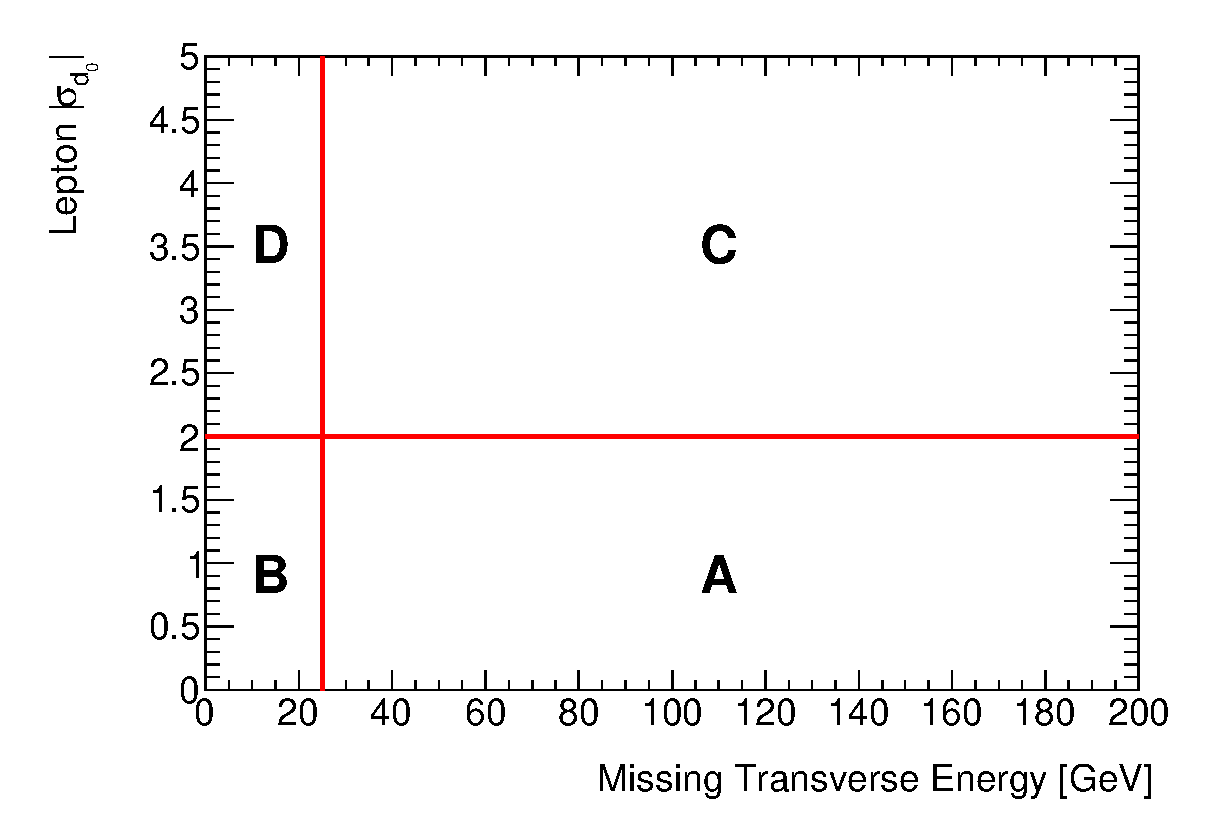
\includegraphics[width=0.9\textwidth]{figures/multijet/abcdExample_met_vs_d0sigBL20}
\end{center}
\caption{A pictoral representation of the four regions used in the
  ABCD calculation.} \label{fig:abcdCartoon}
\end{figure}
Assuming that the two variables chosen to define the ABCD regions are completely uncorrelated, the 
yield of the process being modeled (QCD multi-jets in this case) in the A region is given by
\begin{equation}
N_{A} = N_C \frac{N_B}{N_D}
\label{eq:simpleABCD}
\end{equation}
where the yields $N_i$ are yields calculated from data - all Monte Carlo backgrounds (\ttbar, 
W/Z+jets, single top, diboson processes) in region $i$ ($N_i = N_i^{\text{data}} - N_i^{\text{MC Bkgs}}$). 
The assumption underlying Equation~\ref{eq:simpleABCD} is that the relationship between the 
yields in the B and D regions is the same as the relationship between the A and C regions, i.e.
\begin{equation}
\frac{N_{A}}{N_{C}} = \frac{N_B}{N_D}
\label{eq:correlationStatement}
\end{equation}
Using equation ~\ref{eq:correlationStatement}, the quantity $R= \frac{N_{C} N_B}{N_{A} N_D}$ can be 
defined. In the case of two completely uncorrelated variables, $R=1$ and the ABCD estimation reduces 
to Equation~\ref{eq:simpleABCD}. If the two variables are not completely uncorrelated, the $R$ 
factor enters as a correction to Equation~\ref{eq:simpleABCD} for the multi-jet estimation in the A 
region, and the expression can be rewritten as
\begin{equation}
N_{A} = R \frac{N_C N_B}{N_D}
\label{eq:advancedABCD}
\end{equation}
The $R$ factor is calculated for each selection (\emph{non-res}, \emph{low-mass}, and \emph{high-mass}) individually,
and the results at each step of the selection is provided in
Table~\ref{tab:rValues}.


\begin{table}[h!]
\centering
\begin{tabular}{c|c|c|c}
\hline\hline
\multicolumn{4}{c}{QCD $R$ Values, Non-resonant Selection}\\\hline\hline
mww 	& bbpt210 	& bbpt300 	& wwpt250	\\\hline 
0.74 $\pm$ 0.04 	& 0.79 $\pm$ 0.23 	& 1.07 $\pm$ 1.18 	& ---	\\\hline \hline
%\end{tabular}

\multicolumn{4}{c}{QCD $R$ Values, Low Mass Selection (m500)}\\\hline\hline
mww 	& bbpt210 	& wwpt150 	& hh500	\\\hline 
0.74 $\pm$ 0.04 	& 0.79 $\pm$ 0.23 	& --- 	& ---	\\\hline \hline

%\begin{tabular}{c|c|c|c}
\multicolumn{4}{c}{QCD $R$ Values, Low Mass Selection (m700)}\\\hline\hline
mww 	& bbpt210 	& wwpt250 	& hh700	\\\hline 
0.74 $\pm$ 0.04 	& 0.79 $\pm$ 0.23 	& 0.09 $\pm$ 0.14 	& ---	\\\hline \hline
%\end{tabular}

%\begin{tabular}{c|c|c|c}
\multicolumn{4}{c}{QCD $R$ Values, High Mass Selection}\\\hline\hline
bbpt350 	& wwpt250 	& drww15 	& hh2000	\\\hline 
0.48 $\pm$ 0.09 	& 0.43 $\pm$ 0.08 	& 0.50 $\pm$ 0.16 	& 4.28 $\pm$ 5.30	\\\hline 
\hline\hline
\end{tabular}


\caption[Values of R at each selection]{Values calculated for $R$ at each stage in the \emph{non-res},
  \emph{low-mass}, and \emph{high-mass} selections. The estimate of multi-jet
  contribution in the A region uses the $R$ value calculated after the
  first criteria of each selection.} \label{tab:rValues}
\end{table}
In order to minimize the statistical error on $R$, the $R$ value calculated after 
the first criteria of each selection (0.74 and 0.48) is used in Equation~\ref{eq:advancedABCD} to estimate the multi-jet
background after each subsequent selection. This can be done given the
compatibility of the $R$ value at the end of the cutflow with that at
the point where $R$ is evaluated. In order to check such compatibility
with higher statistics, the $R$ value has been calculated applying
each selection just after $R$ is evaluated, in order
to check that $R$ is not correlated with each of the selections.
The result is shown in Table \ref{tab:R_after_X}.

\begin{table}[h!]
\centering

\begin{tabular}{c|c|c|c}
\hline\hline

\multicolumn{4}{c}{QCD $R$ Values, Non-resonant Selection}\\\hline\hline
mww 	                & mww + bbpt210 	& mww + bbpt300 	& mww + wwpt250 	\\\hline 
0.74 $\pm$ 0.04 	& 0.79 $\pm$ 0.23 	& 1.12 $\pm$ 1.22 	& 0.25 $\pm$ 0.20 	\\\hline \hline
\multicolumn{4}{c}{QCD $R$ Values, Low Mass (m500) Selection}\\\hline\hline
mww 	                & mww + bbpt210 	& mww + wwpt150 	& mww + hh500	  \\\hline 
0.74 $\pm$ 0.04 	& 0.79 $\pm$ 0.23 	& 0.50 $\pm$ 0.08 	& 0.52 $\pm$ 0.09  \\\hline \hline
\multicolumn{4}{c}{QCD $R$ Values, Low Mass (m700) Selection}\\\hline\hline
mww 	                & mww + bbpt210 	& mww + wwpt250 	& mww + hh700	  \\\hline 
0.74 $\pm$ 0.04 	& 0.79 $\pm$ 0.23 	& 0.25 $\pm$ 0.20 	& 0.63 $\pm$ 0.13  \\\hline \hline
\multicolumn{4}{c}{QCD $R$ Values, High Mass Selection}\\\hline\hline
bbpt350 	        & bbpt350 + wwpt250 	& bbpt350 + drww15 	& bbpt350 + hh2000	\\\hline 
0.47 $\pm$ 0.06 	& 0.44 $\pm$ 0.08 	& 0.52 $\pm$ 0.17	& 1.07 $\pm$ 0.67 	\\\hline 

\hline\hline
\end{tabular}

\caption[Cross check for coorelation with R]{Values of $R$ obtained applying a single selection after $R$ is nominally evaluated.} \label{tab:R_after_X}
\end{table}


Once the normalization of the multi-jet background in the A region is calculated using Equation~\ref{eq:advancedABCD}, the shape of the multi-jet template is taken from the data minus Monte Carlo distribution in the C region since the two are kinematically identical except for \dsig.

The uncertainty due to the limited statistics in the B and D regions is the
main source of the multi-jet estimation method systematics. In order to minimise
such error,  the yields from the  B and D regions used in the ABCD
calculation are frozen at a level of the cutflow to minimise statistical fluctuations.
The B and D region yields are frozen after the \ptbb $>$ 210 GeV for the \emph{non-res} and \emph{low-mass} selection, and after the $p_{T}(WW)>$ 250 GeV for the \emph{high-mass} selection. Appendix~\ref{app:qcd_BDregionStudy_appendix} details the study carried out to select the stage at which to freeze the B and D regions. 

To further reduce the error coming from the C region, the shape of the data minus Monte Carlo, i.e. non-prompt, 
\mbb distribution was studied as a function of each individual criteria for each selection. If the \mbb shape is 
unchanged by the additions of further kinematic selections, the C region shape can be taken from an 
earlier stage in the cutflow, reducing the shape uncertainty and overall statistical error on the QCD yield.
To determine the stability of the \mbb shape, the ratio of events in the \mbb signal region ([100, 140] GeV)
over the numbers of events in the full \mbb spectrum was computed for each individual criteria using the C region 
of the ABCD method. This ratio was found to be stable across each selection, and the results of this 
calculation are provided in Table~\ref{tab:efficiencyFactor}. 

  \begin{table}[h!]%\fontsize{8}{9}\selectfont
    \centering
    \begin{tabular}{c|c|c|c}
      \hline\hline
      \multicolumn{4}{c}{reOptNonRes: \mbb SR/Total Ratios For Individual Selections}\\\hline\hline 
      mww 	& bbpt210 	& bbpt300 	& wwpt250 	\\\hline 
      0.17 $\pm$ 0.02 	& 0.15 $\pm$ 0.03 	& 0.13 $\pm$ 0.05 	& 0.16 $\pm$ 0.05 	\\\hline 
    \end{tabular}
    \vspace{5pt}
    
    \begin{tabular}{c|c|c|c}
      \hline\hline
      \multicolumn{4}{c}{reOpt500: \mbb SR/CR Ratios For Individual Selections}\\\hline\hline 
      mww 	& bbpt210 	& wwpt150 	& hh500 	\\\hline 
      0.17 $\pm$ 0.02 	& 0.15 $\pm$ 0.03 	& 0.18 $\pm$ 0.02 	& 0.22 $\pm$ 0.03 	\\\hline 
    \end{tabular}
    \vspace{5pt}

    \begin{tabular}{c|c|c|c}
      \hline\hline
      \multicolumn{4}{c}{reOpt700: \mbb SR/Total Ratios For Individual Selections}\\\hline\hline 
      mww 	& bbpt210 	& wwpt250 	& hh700 	\\\hline 
      0.17 $\pm$ 0.02 	& 0.15 $\pm$ 0.03 	& 0.16 $\pm$ 0.05 	& 0.16 $\pm$ 0.02 	\\\hline 
    \end{tabular}
    \vspace{5pt}

    \begin{tabular}{c|c|c|c}
      \hline\hline
      \multicolumn{4}{c}{reOpt2000: \mbb SR/Total Ratios For Individual Selections}\\\hline\hline 
      bbpt350 	& wwpt250 	& drww15 	& hh2000 	\\\hline 
      0.12 $\pm$ 0.08 	& 0.16 $\pm$ 0.05 	& 0.19 $\pm$ 0.02 	& 0.11 $\pm$ 0.14 	\\\hline 
      \hline 
    \end{tabular}
    \caption[Ratio of events in SR over SR+CR]{The ratio of events in the \mbb signal region ([100, 140] GeV) over the numbers of events in the full \mbb spectrum for each individual selection. Both event yields are calculated in the C region of the ABCD method. The ratios are found to be stable across each selection.}        \label{tab:efficiencyFactor}
  \end{table}

The normalized shapes of the full \mbb distributions after each 
selection are shown in Figure~\ref{fig:mbbShapes}. The earliest selection with a consistent shape was chosen as the
shape for each cutflow and this corresponds to the shape obtained
after the  \ptbb $>$ 210 GeV for the non-resonant the m500 and m700  selections,  and after the  \ptww $>$ 250 GeV for the m2000 selection.

\begin{figure}[h!]
\begin{center}
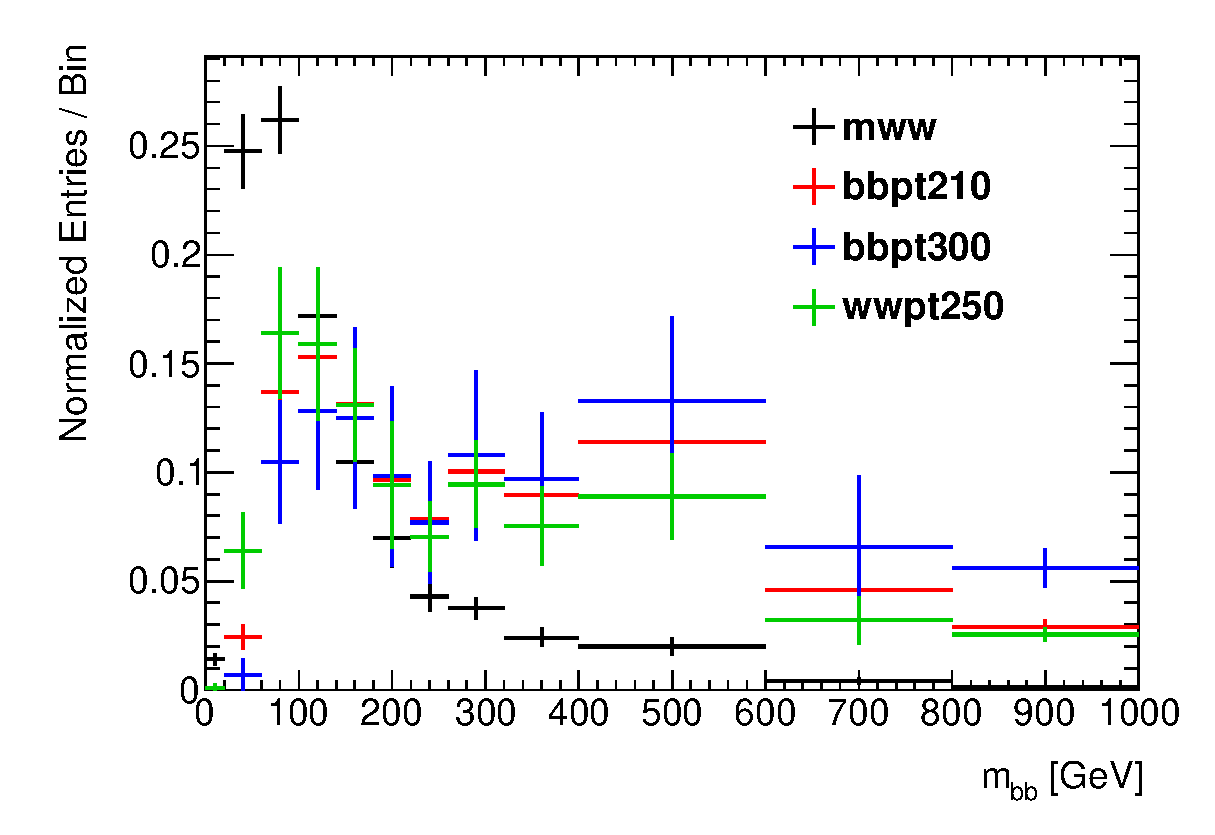
\includegraphics[width=0.49\textwidth]{figures/multijet/reOptNonRes_mbbShape_individualCuts_elmu}
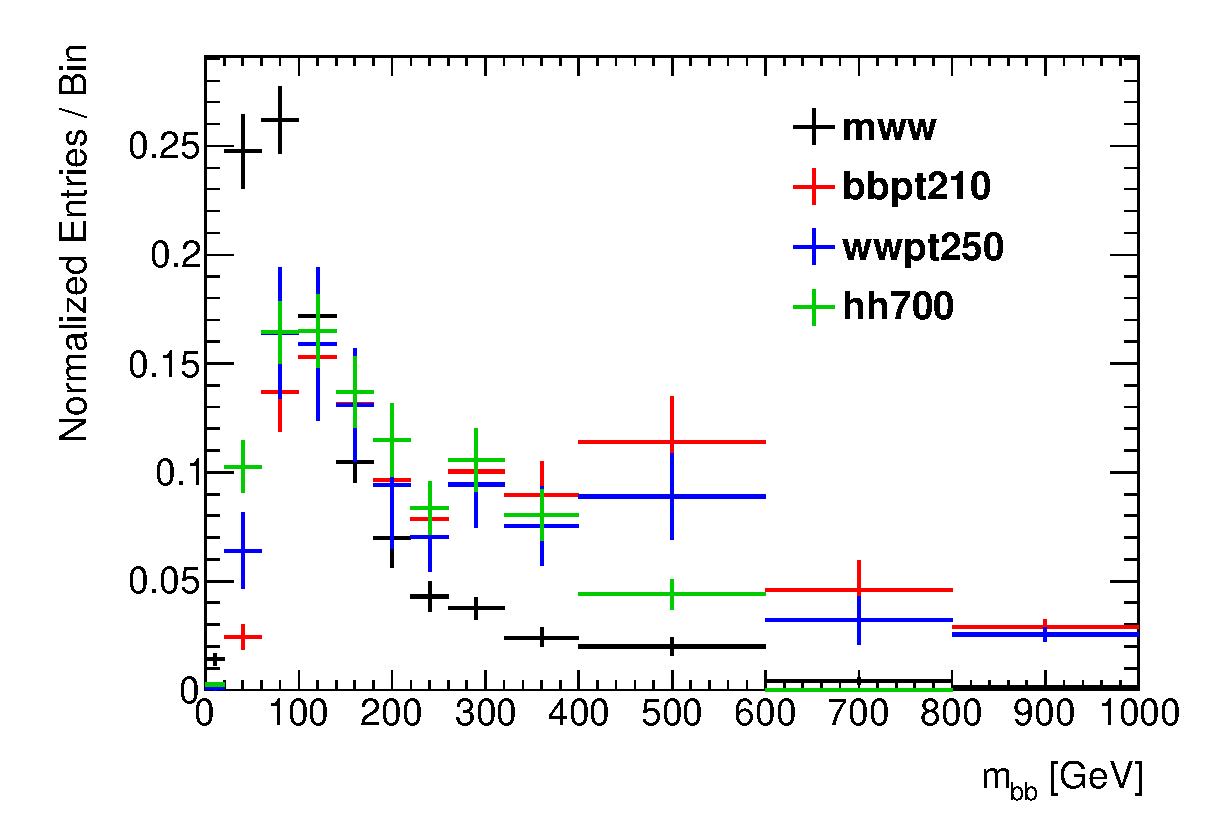
\includegraphics[width=0.49\textwidth]{figures/multijet/reOpt700_mbbShape_individualCuts_elmu}
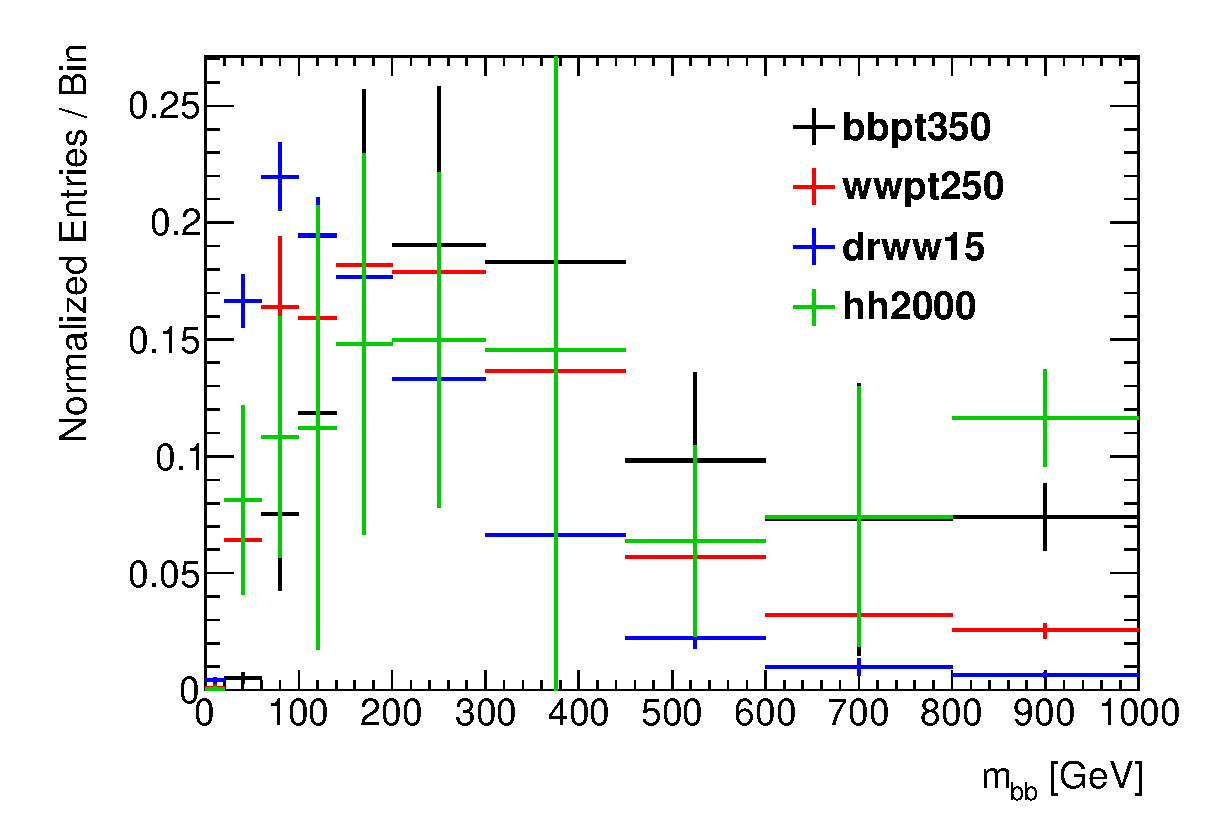
\includegraphics[width=0.49\textwidth]{figures/multijet/reOpt2000_mbbShape_individualCuts_elmu}
\end{center}

\caption[The normalized shapes of the full \mbb distributions]{The normalized shapes of the full \mbb distributions after
  each in each selection. Shapes from the non-resonant cutflow are
  shown at the top left, shapes from the \emph{low-mass} selection are shown
  at the top left, and shapes from the \emph{high-mass} selection are shown
  at the bottom. The earliest selection with a consistent shape
  was chosen as the shape for each cutflow and this corresponds to the
  shape obtained after the \mww and \ptbb $>$ 210 GeV for the
  \emph{non-res} and \emph{low-mass} selections and after the \ptbb $>$ 350 GeV
  and \ptww $>$ 250 GeV for the \emph{high-mass} mass selection.} \label{fig:mbbShapes}
\end{figure}

Since \ttbar and  multi-jet contaminate the control
regions used for their estimation,  additional studies were
performed via an iterative procedure to ensure that the \ttbar and QCD
yields converge to stable values and that the estimation technique is
able to disentangle between the two backgrounds.
Appendix~\ref{app:qcd_ttbarNFstability_appendix} details the results of the study, and the yields 
were found to converge (stable within $<5\%$) after a few iterations for each cutflow.

%Since the \mtw distribution should contain a large multi-jet contribution at low \mtw, the agreement 
%between data and prediction in the \mtw distribution for each selection acts as a closure test on 
%the estimation of the multi-jet background by the ABCD method. Appendices~\ref{app:data_exp_reOptNonRes}
%,~\ref{app:data_exp_reOpt700}, and~\ref{app:data_exp_reOpt2000} show these distributions in the 
%\ttbar control regions for each selection. Good agreement is observed.

To evaluate the systematic error of the estimation, a Sherpa multi-jet $bb$ sample is used to compare 
the ABCD prediction to the Monte Carlo expectation using events with exactly one lepton and four jets. 
No $b$-tagging requirements or other event selection criteria are applied. Pseudo-data is produced using
the multi-jet Monte Carlo and events from the nominal \ttbar Monte Carlo. The $R$ factor is calculated
using the inclusive $b$-tag (0, 1, or 2 $b$-tags) and used to estimate the QCD contribution in the two
$b$-tag exclusive region. The percent difference between the number of events from the ABCD estimation 
and the number of multi-jet events from Monte Carlo used to produce the pseudo-data is taken as the 
systematic uncertainty. This uncertainty is calculated to be 36\%. In addition, the $bb$ MC is used to
calculate the $R$ factor for each selection (\emph{non-res}, \emph{low-mass}, and \emph{high-mass}) and each lepton 
channel, and the results at each kinematic criteria in each selection are provided in the Table~\ref{tab:lepR}. 

\begin{table}[h!]
\centering
\begin{tabular}{c|c|c|c|c}

\hline\hline
\multicolumn{5}{c}{Non-resonant: QCD $R_{non-prompt}$ Values}\\\hline\hline 
          & mww                 & bbpt210 	        & bbpt300 	        & wwpt250	        \\ \hline 
Combined  & 0.74 $\pm$ 0.04 	& 0.80 $\pm$ 0.05  	& 0.64 $\pm$ 0.08 	& 0.62 $\pm$ 0.05	\\\hline 
Electrons & 0.72 $\pm$ 0.05  	& 0.75 $\pm$ 0.06 	& 0.68 $\pm$ 0.10 	& 0.64 $\pm$ 0.06	\\\hline 
Muons     & 0.81 $\pm$ 0.06 	& 0.92 $\pm$ 0.11 	& 0.55 $\pm$ 0.15 	& 0.59 $\pm$ 0.10	\\\hline 
\hline\hline
\multicolumn{5}{c}{Low-mass (m500): QCD $R_{non-prompt}$ Values}\\\hline\hline 
          & mww                 & bbpt210 	        & wwpt150 	        & hh500 	        \\ \hline 
Combined  & 0.74 $\pm$ 0.04 	& 0.80 $\pm$ 0.05 	& 0.68 $\pm$ 0.03  	& 0.50 $\pm$ 0.03	\\\hline 
Electrons & 0.72 $\pm$ 0.05 	& 0.75 $\pm$ 0.06 	& 0.65 $\pm$ 0.03 	& 0.44 $\pm$ 0.04	\\\hline 
Muons     & 0.81 $\pm$ 0.06 	& 0.92 $\pm$ 0.11 	& 0.75 $\pm$ 0.06 	& 0.58 $\pm$ 0.07	\\\hline 
\hline\hline

\multicolumn{5}{c}{Low-mass (m700): QCD $R_{non-prompt}$ Values}\\\hline\hline 
          & mww                 & bbpt210 	        & wwpt250 	        & hh700 	        \\ \hline 
Combined  & 0.74 $\pm$ 0.04 	& 0.80 $\pm$ 0.05 	& 0.62 $\pm$ 0.25 	& 0.60 $\pm$ 0.03	\\\hline 
Electrons & 0.72 $\pm$ 0.05 	& 0.75 $\pm$ 0.06 	& 0.64 $\pm$ 0.06 	& 0.52 $\pm$ 0.04	\\\hline 
Muons     & 0.81 $\pm$ 0.06 	& 0.92 $\pm$ 0.11 	& 0.59 $\pm$ 0.10 	& 0.74 $\pm$ 0.08	\\\hline 
\hline\hline


\multicolumn{5}{c}{High-mass: QCD $R_{non-prompt}$ Values}\\\hline\hline 
          & bbpt350             & wwpt250 	        & drww15 	        & hh2000 	        \\ \hline 
Combined  & 0.47 $\pm$ 0.09 	& 0.62 $\pm$ 0.05 	& 0.68 $\pm$ 0.03 	& 0.58 $\pm$ 0.13	\\\hline 
Electrons & 0.48 $\pm$ 0.10 	& 0.64 $\pm$ 0.06 	& 0.60 $\pm$ 0.04 	& 0.57 $\pm$ 0.14	\\\hline 
Muons     & 0.44 $\pm$ 0.20 	& 0.59 $\pm$ 0.10 	& 0.82 $\pm$ 0.07 	& 0.65 $\pm$ 0.39	\\\hline 
\hline\hline


\end{tabular}
\caption[$R_{non-prompt}$]{$R_{non-prompt}$ calculated for the QCD Monte Carlo sample at using each kinematic criteria individually from all selections. The lepton channels are shown separated and combined.}
\label{tab:lepR}
\end{table}










\subsection{Background Shape and Cutflow}
\label{sec:systematics}
 The modeling of the background was checked at all selection
stages and, in general, shows good agreement with data.
Figure~\ref{fig:resolved_mtlep} shows the $\mT$ distribution of the
leptonic $W$ boson candidate  in the three
top control regions. The $\mT$ variable is defined as:
\[
\mT = \sqrt{2\pt^{\ell}\met\cdot (1-\rm{cos}\Delta \phi)} ~,
\]
where $\Delta \phi$ is the azimuthal
angle between $\pt^{\ell}$ and $\met$. The multijet background populates the
low values of the $\mT$ distribution, so any mis-modeling of the multijet background would be clearly visible in the $\mT$ distribution.
%QCD multijet background is estimated in each top control region following the ABCD method described above.
 
\begin{figure}
%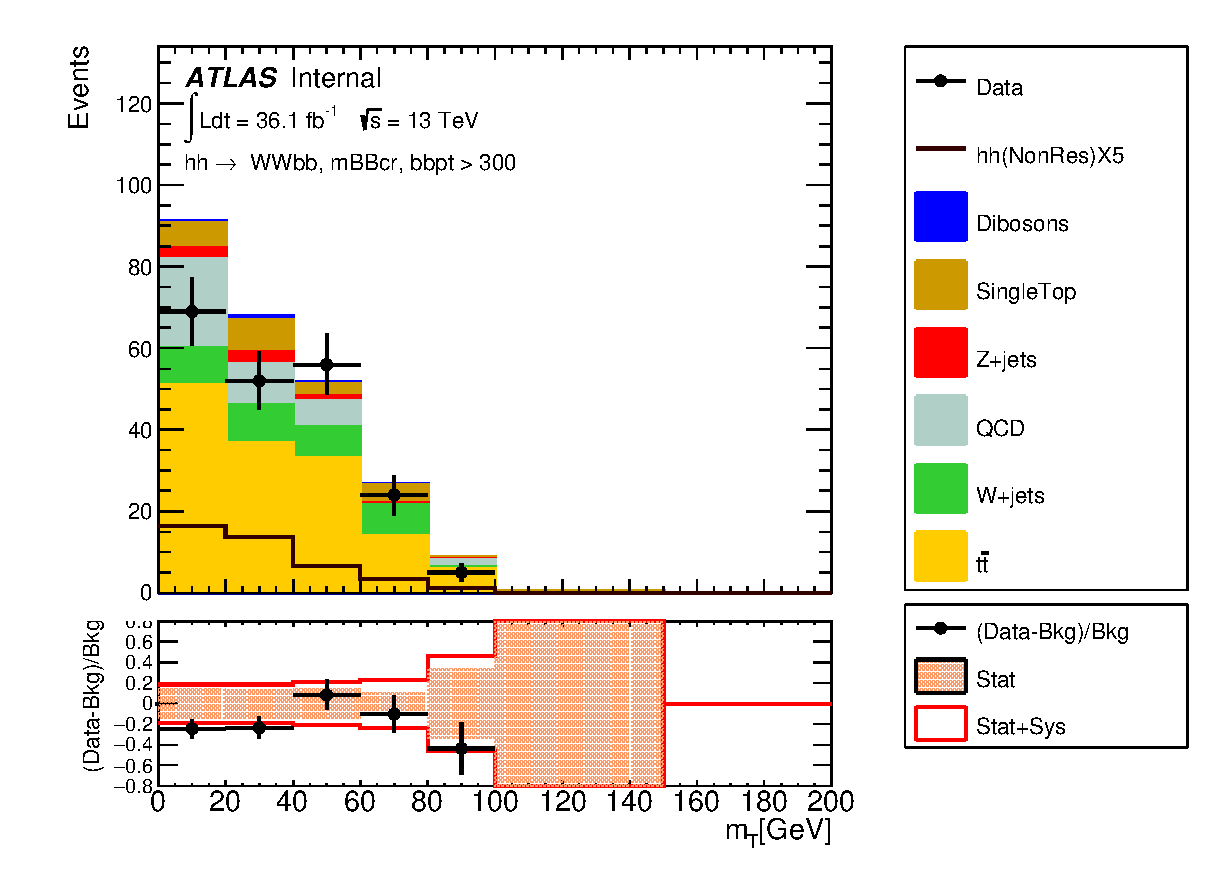
\includegraphics[width=0.45\textwidth, height=0.35\textwidth]{figures/C_reOptNonRes_mww_bbpt210_bbpt300_wlepmtben_regionA_met25d020}
\includegraphics*[width=0.5\textwidth]{paper_figures/C_mBBcr_reOptNonRes_mww_bbpt210_bbpt300_wlepmtben_regionA_met25d020.eps}
%\includegraphics*[width=0.3\textwidth]{figures/C_mBBcr_reOpt500_mww_bbpt210_wlepmtben_regionA_met25d020.eps}
\includegraphics*[width=0.5\textwidth]{paper_figures/C_mBBcr_reOpt700_mww_bbpt210_wlepmtben_regionA_met25d020.eps}
\includegraphics*[width=0.5\textwidth]{paper_figures/C_mBBcr_reOpt2000_bbpt350_wlepmtben_regionA_met25d020.eps}
\caption[The $\mT$ distribution]{The $\mT$ distribution in the three top-background control regions for the \emph{non-res}, \emph{low-mass}, and
 the \emph{high-mass} selections of the resolved analyses.
  %The signal
  %distributions shown are for the  SM non-resonant signal scaled with a factor
  %300 (top-left), and  for the resonant signals with mass 1000~GeV (top-right) and 2000~GeV
  %(bottom) scaled to the expected upper limit cross section reported
  %in Section \ref{sec:MainResults}.
  The signal contamination is negligible, and hence not shown. The lower panel shows the
  fractional difference between the data and the total expected background
  with the corresponding statistical and total uncertainty. }
  \label{fig:resolved_mtlep}
\end{figure}
 
 
Figures~\ref{fig:mbb_1} and ~\ref{fig:mbb_2} show the $m_{b \bar{b}}$ distributions at the
selection stage where all requirements, including $m_{HH}$, are applied except the one on $m_{b \bar{b}}$ itself.
The expected background is in agreement with the data over the entire distribution, and  
close to the signal region in particular. All simulated backgrounds are normalized according to their theoretical cross-sections, except \ttbar, which is normalized in the top CRs.
 
\begin{figure}
\begin{flushleft}
%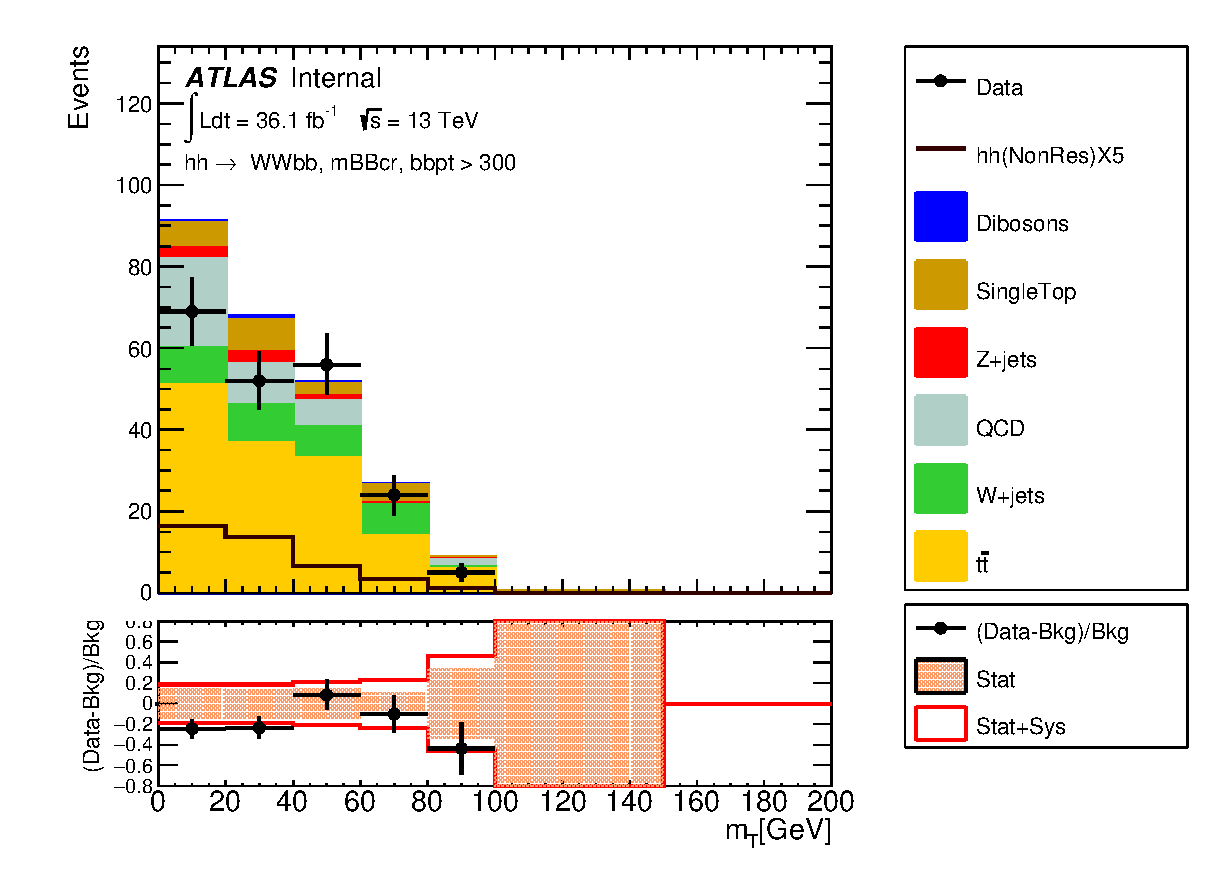
\includegraphics[width=0.45\textwidth, height=0.35\textwidth]{figures/C_reOptNonRes_mww_bbpt210_bbpt300_wlepmtben_regionA_met25d020}
\includegraphics*[width=0.49\textwidth]{paper_figures/C_reOptNonRes_mww_bbpt210_bbpt300_wwpt250_bbMass_regionA_met25d020.eps}
\includegraphics*[width=0.49\textwidth]{paper_figures/C_reOpt500_mww_bbpt210_wwpt150_hh500_bbMass_regionA_met25d020.eps}
\end{flushleft}
\caption[The $m_{b \bar{b}}$ distribution]{The $m_{b \bar{b}}$ distribution in the resolved analysis for the \emph{non-res} and \emph{m500} selections at the end of the
 selection sequence, before applying the $m_{b \bar{b}}$ requirement. The signals shown
 are from SM non-resonant $HH$ production scaled up by a factor of 300 (left) and from a scalar resonance with mass 500~\GeV\ scaled to the expected upper-limit
 cross section reported in Section~\ref{sec:results} (right).  The lower panel shows the fractional difference
  between data and the total expected background
 with the corresponding statistical and total uncertainty.
} \label{fig:mbb_1}
\end{figure}
 
\begin{figure}
\begin{flushleft}
\includegraphics*[width=0.49\textwidth]{paper_figures/C_reOpt700_mww_bbpt210_wwpt250_hh1000_bbMass_regionA_met25d020.eps}
\includegraphics*[width=0.49\textwidth]{paper_figures/C_reOpt2000_bbpt350_wwpt250_drww15_hh2000_bbMass_regionA_met25d020.eps}
\end{flushleft}
\caption[The $m_{b \bar{b}}$ distribution]{The $m_{b \bar{b}}$ distribution in the resolved analysis for the
 \emph{low-mass} and \emph{high-mass} selections at the end of the
 selection sequence, before applying the $m_{b \bar{b}}$ requirement. The signals shown
 are from scalar resonances with mass 1000~\GeV\ (left) and 2000~\GeV\ (right)
 scaled to the expected upper-limit cross section reported in
 Section~\ref{sec:results}.  The lower panel shows the fractional difference
  between data and the total expected background
 with the corresponding statistical and total uncertainty.} \label{fig:mbb_2}
\end{figure}
 
%\begin{figure}
%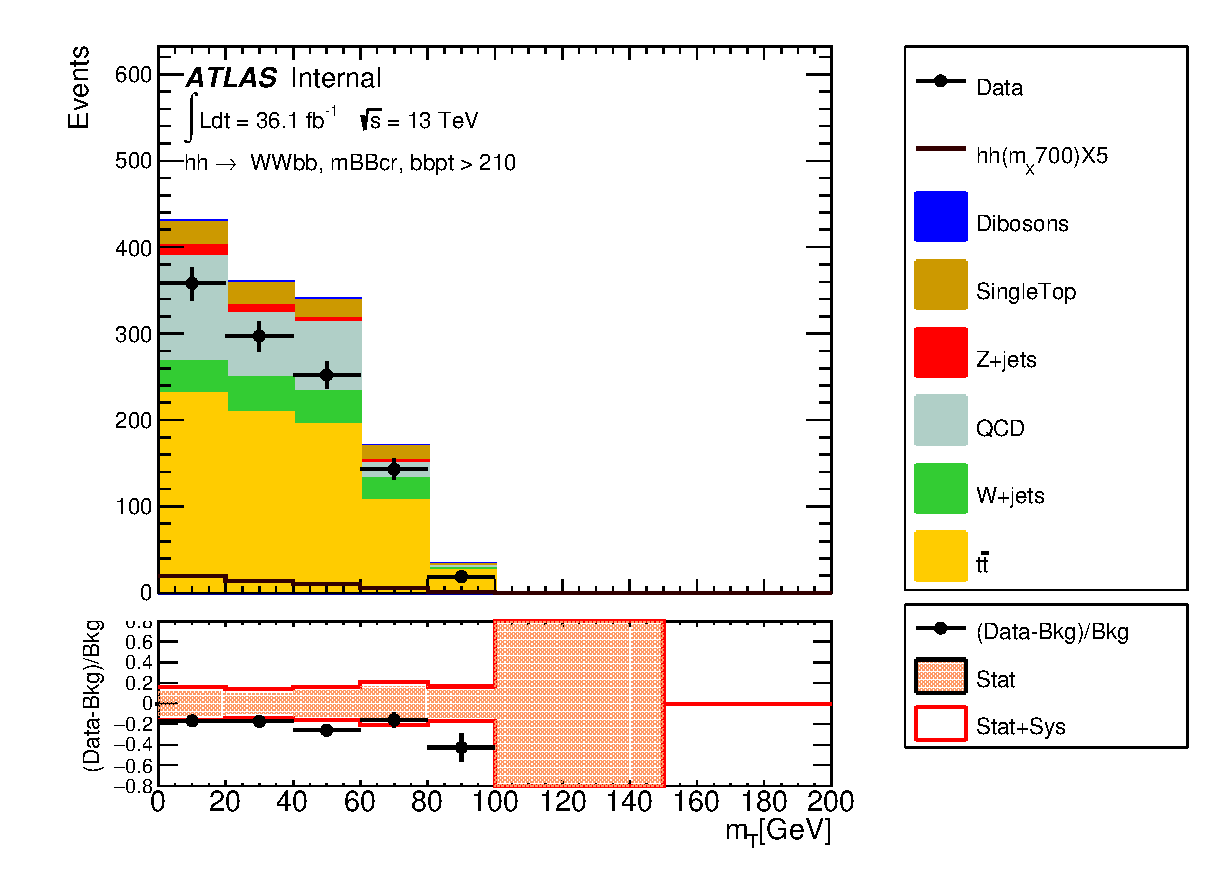
\includegraphics[width=0.45\textwidth, height=0.35\textwidth]{figures/C_reOpt700_mww_bbpt210_wlepmtben_regionA_met25d020}
%\includegraphics*[width=0.45\textwidth]{figures/C_reOpt700_mww_bbpt210_bbMass_regionA_met25d020}
%\caption{$m_{T}$ and $m_{bb}$ distributions for low-mass selection after requiring $p_{T}(bb) > 210$ GeV. The lower panel shows the agreement between data and expected backgrounds and the uncertainties on the total backgrounds. Signal has been arbitrarily scaled to show the shape.}
%\label{fig:mt_mbb_low}
%\end{figure}
 
%\begin{figure}
%\label{fig:mt_mbb_high}
%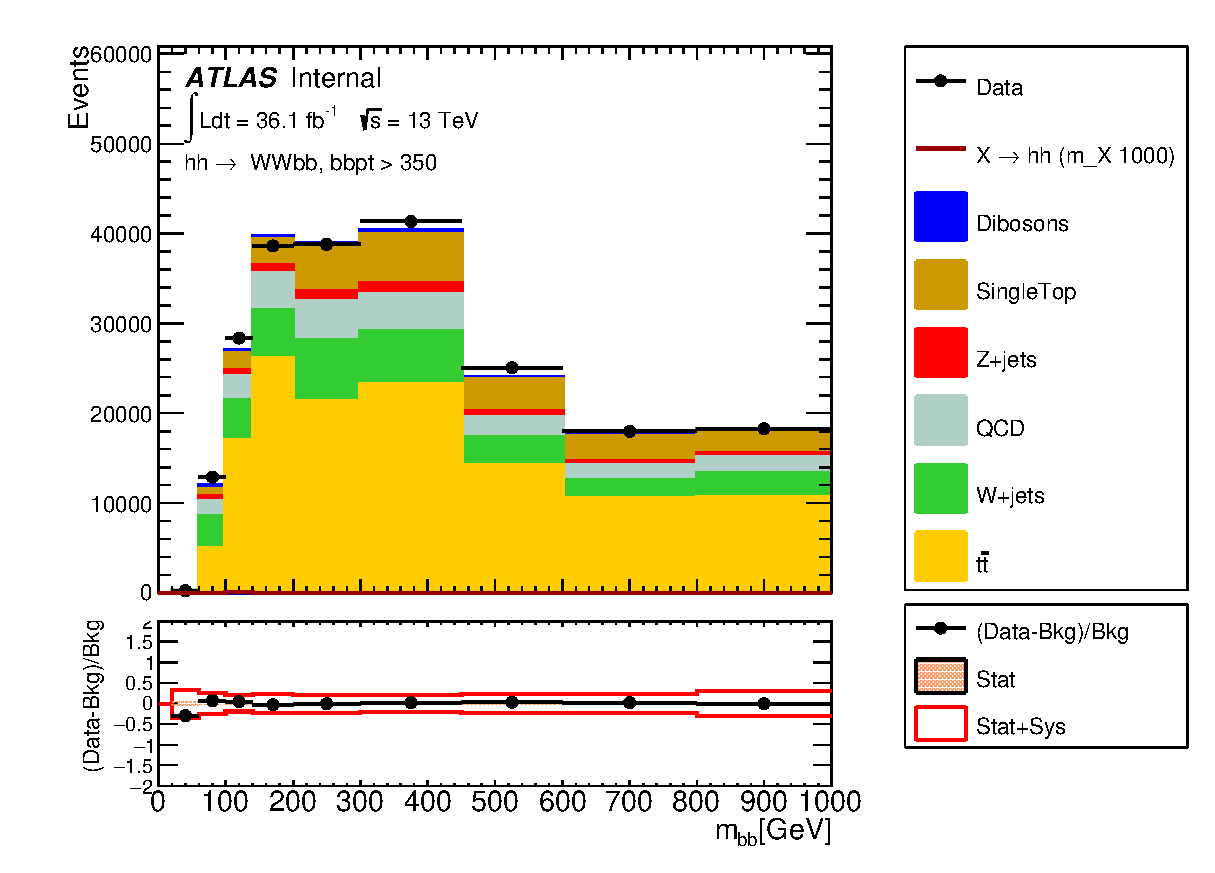
\includegraphics[width=0.45\textwidth, height=0.35\textwidth]{figures/C_reOpt2000_bbpt350_bbMass_regionA_met25d020}
 
%\caption{$m_{T}$ and $m_{bb}$ distributions for high-mass selection after requiring $p_{T}(bb) > 350$ GeV. The lower panel shows the agreement between data and expected backgrounds and the un%certainties on the total backgrounds. Signal has been arbitrarily scaled to show the shape.}
%\end{figure}
 
\begin{table}
%\fontsize{7}{8}\selectfont
 \begin{tabular}{l|c|c|c|c|c}
\hline\hline

\multicolumn{5}{c}{\textbf{SR}: 100 $<$ \mbb $<$ 140 GeV}\\\hline\hline
Sample  	& mww 	& bbpt210 	& bbpt300 	& wwpt250 	& mbb  \\\hline
\ttbar 	& 7461.0 $\pm$ 48.6 	& 162.9 $\pm$ 7.3 	& 27.9 $\pm$ 2.9 	& 18.4 $\pm$ 2.4 	& 15.4 $\pm$ 2.2	\\\hline 
QCD 	& 2756.2 $\pm$ 210.5 	& 48.7 $\pm$ 14.2 	& 6.6 $\pm$ 1.9 	& 4.2 $\pm$ 1.2 	& 3.6 $\pm$ 1.6	\\\hline 
Wv221 	& 640.8 $\pm$ 12.7 	& 19.1 $\pm$ 1.4 	& 5.0 $\pm$ 0.6 	& 3.1 $\pm$ 0.5 	& 2.3 $\pm$ 0.4	\\\hline 
SingleTop 	& 452.2 $\pm$ 9.6 	& 14.3 $\pm$ 1.7 	& 1.7 $\pm$ 0.5 	& 1.0 $\pm$ 0.4 	& 0.6 $\pm$ 0.3	\\\hline 
Dibosonsv221 	& 21.6 $\pm$ 1.3 	& 0.6 $\pm$ 0.2 	& 0.4 $\pm$ 0.2 	& 0.0 $\pm$ 0.0 	& 0.0 $\pm$ 0.0	\\\hline 
Zv221 	& 262.8 $\pm$ 4.4 	& 3.1 $\pm$ 0.3 	& 1.0 $\pm$ 0.2 	& 0.2 $\pm$ 0.1 	& 0.2 $\pm$ 0.1	\\\hline 
\hline
Background Sum 	& 11594.7$\pm$ 216.7 	& 248.6$\pm$ 16.1 	& 42.6$\pm$ 3.6 	& 27.0$\pm$ 2.8 	& 22.1$\pm$ 2.8	\\\hline 
\hline
XhhSM 	& 68.3 $\pm$ 2.4 	& 20.7 $\pm$ 0.9 	& 6.7 $\pm$ 0.4 	& 5.5 $\pm$ 0.3 	& 4.8 $\pm$ 0.3	\\\hline 
Data 	& 11450.0 	& 232.0 	& 47.0 	& 31.0 	& 22.0	\\\hline 
\end{tabular}
\caption[Number of SR events in the non-res selection]{ The number of expected background and signal events in the
  $m_{bb}$ SR for the non-resonant selection. Only statistical uncertainties are shown. No NF has been applied.} 
\label{tab:nonresSRyields}
\end{table}

%%%%%%%%%%%%%%%%%%%
\begin{center}
\begin{table}
%\fontsize{7}{8}\selectfont
\begin{tabular}{l|c|c|c|c|c}
\hline\hline
\multicolumn{5}{c}{\textbf{SR}: 100 $<$ \mbb $<$ 140 GeV}\\\hline\hline
Sample  	& mww 	& bbpt210 	& wwpt150 	& hh500 	& mbb  \\\hline
\ttbar 	& 7461.0 $\pm$ 48.6 	& 162.9 $\pm$ 7.3 	& 141.7 $\pm$ 6.8 	& 17.3 $\pm$ 2.2 	& 12.6 $\pm$ 1.9	\\\hline 
QCD 	& 2756.2 $\pm$ 210.5 	& 48.7 $\pm$ 14.2 	& 40.2 $\pm$ 11.7 	& 3.3 $\pm$ 1.0 	& 2.9 $\pm$ 1.3	\\\hline 
Wv221 	& 640.8 $\pm$ 12.7 	& 19.1 $\pm$ 1.4 	& 15.3 $\pm$ 1.3 	& 0.1 $\pm$ 0.0 	& -0.2 $\pm$ 0.1	\\\hline 
SingleTop 	& 452.2 $\pm$ 9.6 	& 14.3 $\pm$ 1.7 	& 12.2 $\pm$ 1.6 	& 3.6 $\pm$ 0.8 	& 2.8 $\pm$ 0.7	\\\hline 
Dibosonsv221 	& 21.6 $\pm$ 1.3 	& 0.6 $\pm$ 0.2 	& 0.5 $\pm$ 0.2 	& 0.1 $\pm$ 0.0 	& 0.1 $\pm$ 0.0	\\\hline 
Zv221 	& 262.8 $\pm$ 4.4 	& 3.1 $\pm$ 0.3 	& 1.9 $\pm$ 0.2 	& 0.5 $\pm$ 0.1 	& 0.4 $\pm$ 0.1	\\\hline 
\hline
Background Sum 	& 11594.7$\pm$ 216.7 	& 248.6$\pm$ 16.1 	& 211.8$\pm$ 13.7 	& 24.9$\pm$ 2.5 	& 18.6$\pm$ 2.4	\\\hline 
\hline
Xhh500 	& 6.6 $\pm$ 0.2 	& 1.9 $\pm$ 0.1 	& 1.7 $\pm$ 0.1 	& 0.9 $\pm$ 0.1 	& 0.8 $\pm$ 0.1	\\\hline 
Data 	& 11450.0 	& 232.0 	& 194.0 	& 32.0 	& 26.0	\\\hline 
\end{tabular}
\caption[Number of SR events in the m500 selection]{ The number of expected background and signal events in the  $m_{bb}$ SR for the low-mass selection, m500. Only statistical uncertainties are shown. No NF has been applied.} 
\end{table}
\end{center}


%%%%%%%%%%%%%%%%

\begin{center}
\begin{table}
%\fontsize{7}{8}\selectfont
\begin{tabular}{l|c|c|c|c|c}
\hline\hline
%\multicolumn{5}{c}{\textbf{CR}: \mbb Sideband}\\\hline\hline
\multicolumn{5}{c}{\textbf{SR}: 100 $<$ \mbb $<$ 140 GeV}\\\hline\hline
Sample  	& mww 	& bbpt210 	& wwpt250 	& hh700 	& mbb  \\\hline
\ttbar 	& 7461.0 $\pm$ 48.6 	& 162.9 $\pm$ 7.3 	& 61.5 $\pm$ 4.7 	& 21.9 $\pm$ 2.7 	& 15.3 $\pm$ 2.2	\\\hline 
QCD 	& 2756.2 $\pm$ 210.5 	& 48.7 $\pm$ 14.2 	& 14.1 $\pm$ 4.1 	& 5.5 $\pm$ 1.6 	& 4.8 $\pm$ 2.2	\\\hline 
Wv221 	& 640.8 $\pm$ 12.7 	& 19.1 $\pm$ 1.4 	& 9.7 $\pm$ 1.1 	& 4.1 $\pm$ 0.8 	& 2.6 $\pm$ 0.6	\\\hline 
SingleTop 	& 452.2 $\pm$ 9.6 	& 14.3 $\pm$ 1.7 	& 2.6 $\pm$ 0.7 	& 0.5 $\pm$ 0.2 	& 0.3 $\pm$ 0.2	\\\hline 
Dibosonsv221 	& 21.6 $\pm$ 1.3 	& 0.6 $\pm$ 0.2 	& 0.2 $\pm$ 0.1 	& 0.2 $\pm$ 0.1 	& 0.2 $\pm$ 0.1	\\\hline 
Zv221 	& 262.8 $\pm$ 4.4 	& 3.1 $\pm$ 0.3 	& 0.6 $\pm$ 0.1 	& 0.1 $\pm$ 0.0 	& 0.1 $\pm$ 0.0	\\\hline 
\hline
Background Sum 	& 11594.7$\pm$ 216.7 	& 248.6$\pm$ 16.1 	& 88.7$\pm$ 6.4 	& 32.3$\pm$ 3.2 	& 23.3$\pm$ 3.1	\\\hline 
\hline
Xhh700 	& 9.2 $\pm$ 0.3 	& 7.8 $\pm$ 0.2 	& 5.9 $\pm$ 0.2 	& 5.0 $\pm$ 0.2 	& 4.4 $\pm$ 0.2	\\\hline 
Data 	& 11450.0 	& 232.0 	& 75.0 	& 25.0 	& 22.0	\\\hline 
\end{tabular}
\caption[Number of SR events in the m700 selection]{ The number of expected background and signal events in the  $m_{bb}$ SR for the low-mass selection, m700. Only statistical uncertainties are shown. No NF has been applied.} 
\end{table}
\end{center}

%%%%%%%%%%%%%%%

\begin{center}
\begin{table}
%\fontsize{7}{8}\selectfont
\begin{tabular}{l|c|c|c|c|c}
\hline\hline
\multicolumn{5}{c}{\textbf{SR}: 100 $<$ \mbb $<$ 140 GeV}\\\hline\hline
Sample  	& bbpt350 	& wwpt250 	& drww15 	& hh2000 	& mbb  \\\hline
\ttbar 	& 1307.8 $\pm$ 20.2 	& 1024.9 $\pm$ 17.7 	& 287.5 $\pm$ 9.4 	& 2.2 $\pm$ 0.8 	& 1.4 $\pm$ 0.6	\\\hline 
QCD 	& 207.2 $\pm$ 99.5 	& 191.2 $\pm$ 29.0 	& 55.2 $\pm$ 8.4 	& 2.9 $\pm$ 0.4 	& 2.2 $\pm$ 0.5	\\\hline 
Wv221 	& 341.3 $\pm$ 3.4 	& 291.5 $\pm$ 3.2 	& 110.7 $\pm$ 2.1 	& 4.8 $\pm$ 0.3 	& 3.4 $\pm$ 0.3	\\\hline 
SingleTop 	& 144.1 $\pm$ 5.6 	& 126.6 $\pm$ 5.3 	& 29.2 $\pm$ 2.6 	& 0.5 $\pm$ 0.3 	& 0.5 $\pm$ 0.3	\\\hline 
Dibosonsv221 	& 25.9 $\pm$ 1.5 	& 21.8 $\pm$ 1.3 	& 6.6 $\pm$ 0.7 	& 0.0 $\pm$ 0.0 	& 0.0 $\pm$ 0.0	\\\hline 
Zv221 	& 53.8 $\pm$ 0.8 	& 40.4 $\pm$ 0.7 	& 13.2 $\pm$ 0.4 	& 0.8 $\pm$ 0.1 	& 0.7 $\pm$ 0.1	\\\hline 
\hline
Background Sum 	& 2080.1$\pm$ 101.8 	& 1696.5$\pm$ 34.6 	& 502.5$\pm$ 13.1 	& 11.2$\pm$ 1.0 	& 8.2$\pm$ 0.8	\\\hline 
\hline
Xhh2000 	& 21.0 $\pm$ 0.4 	& 19.3 $\pm$ 0.4 	& 8.4 $\pm$ 0.2 	& 3.4 $\pm$ 0.1 	& 2.9 $\pm$ 0.1	\\\hline 
Data 	& 2182.0 	& 1830.0 	& 587.0 	& 11.0 	& 9.0	\\\hline
\end{tabular}
\caption[Number of SR events in the m2000 selection]{ The number of expected background and signal events in the  $m_{bb}$ SR for the high-mass selection, m2000. Only statistical uncertainties are shown. No NF has been applied.} 
\label{tab:highmassSRyields}
\end{table}
\end{center}

\subsection{Systematic Uncertainties}
This section describes the sources of systematic uncertainties
considered in the analysis. These uncertainties are divided into four
categories: experimental uncertainties, uncertainties on the data
driven background estimation,  uncertainties on the modeling
of background processes estimated from simulation, and theoretical
uncertainties on the signal processes. In the statistical analysis
each systematic uncertainty is treated as a nuisance parameter the
names of which are defined below. These systematic variations are
estimated on the final expected yield in the signal regions.

\subsubsection{Experimental uncertainties}

Each reconstructed object has several sources of uncertainties, each
of which are evaluated separately. Wherever possible, we follow the
latest available recommendations from the ATLAS combined performance (CP)
groups. The leading instrumental uncertainties are
the uncertainty on the $b$-tagging efficiency and the jet energy scale
(JES). The summary of experimental uncertainties is presented in
Table~\ref{tab:syst_summary_sources}.
 
\begin{table}[h]
\centering
\small
\scriptsize
\begin{center}
\begin{tabular}{|l|l|l|l|}
\hline
Source        & Description                          & Analysis Name                         \\ 
\hline
%Muons         & Trigger                                 &    Muons\_Trig                              \\
Muons         & \pt resolution MS                 &   MUON\_MS                           \\ 
Muons         & \pt resolution ID                   &   MUON\_ID                             \\ 
Muons         & \pt scale                               &   MUON\_SCALE                     \\ 
Muons         & Isolation efficiency SF         &   MUON\_ISO\_SYS               \\ 
Muons         & Isolation efficiency SF         &   MUON\_ISO\_STAT              \\ 
Muons         & Reconstruction efficiency SF         &  MUON\_EFF\_SYS             \\ 
Muons         & Reconstruction efficiency SF         &  MUON\_EFF\_STAT           \\ 
Muons         & Trigger efficiency SF            &  MUON\_EFF\_TrigStatUncertainty \\ 
Muons         & Trigger efficiency SF            &  MUON\_EFF\_TrigSystUncertainty  \\ 
%Muons         & TTVA efficiency SF         &   MUON\_TTVA\_SYS              & \\ 
%Muons         & TTVA efficiency SF         &   MUON\_TTVA\_STAT             & \\ 
\hline
Electrons         & \pt resolution                           &   EG\_RESOLUTION\_ALL       \\ 
Electrons         & \pt scale                                  &   EG\_SCALE\_ALL                   \\ 
Electrons         & Isolation efficiency SF             &   EL\_EFF\_Iso\_TOTAL\_1NPCOR\_PLUS\_UNCOR  \\ 
Electrons         & Reconstruction efficiency SF  &   EL\_EFF\_Reco\_TOTAL\_1NPCOR\_PLUS\_UNCOR  \\ 
Electrons         & Trigger efficiency SF               &   EL\_EFF\_Trigger\_TOTAL\_1NPCOR\_PLUS\_UNCOR  \\ 
Electrons         & Identification efficiency SF      &   EL\_EFF\_ID\_TOTAL\_1NPCOR\_PLUS\_UNCOR  \\ 
\hline
Tau	               & Energy scale model			& TAUS\_TRUEHADTAU\_SME\_TES\_MODEL\\
Tau	               & Energy scale detector		& TAUS\_TRUEHADTAU\_SME\_TES\_DETECTOR \\
Tau	               & In-situ energy calibration		& TAUS\_TRUEHADTAU\_SME\_TES\_INSITU \\
\hline
MET           & Soft term                       &   MET\_SoftTrk\_ResoPerp            \\ 
MET           & Soft term                       &   MET\_SoftTrk\_ResoPara            \\ 
MET           & Soft term                       &   MET\_SoftTrk\_Scale              \\ 
\hline
Small-R Jets  & JES strongly reduced            &   JET\_SR1\_JET\_GroupedNP\_1                   \\ 
Small-R Jets  & JES strongly reduced            &   JET\_SR1\_JET\_GroupedNP\_2                   \\ 
Small-R Jets  & JES strongly reduced            &   JET\_SR1\_JET\_GroupedNP\_3                   \\ 
Small-R Jets  & JES strongly reduced            &   JET\_SR1\_JET\_EtaIntercalibration\_NonClosure  \\ 
Small-R Jets  & Energy resolution                  &   JET\_JER\_SINGLE\_NP                               \\ 
Small-R Jets  & JVT efficiency SF                  &   JET\_JvtEfficiency                                                   \\ 
\hline
$b$-tagging     & Flavor tagging scale factors    &    FT\_EFF\_Eigen\_Light\_0                               \\
$b$-tagging     & Flavor tagging scale factors    &    FT\_EFF\_Eigen\_Light\_1                               \\
$b$-tagging     & Flavor tagging scale factors    &    FT\_EFF\_Eigen\_Light\_2                               \\
$b$-tagging     & Flavor tagging scale factors    &    FT\_EFF\_Eigen\_Light\_3                               \\
$b$-tagging     & Flavor tagging scale factors    &    FT\_EFF\_Eigen\_Light\_4                               \\
$b$-tagging     & Flavor tagging scale factors    &    FT\_EFF\_Eigen\_Light\_5                               \\
$b$-tagging     & Flavor tagging scale factors    &    FT\_EFF\_Eigen\_Light\_6                               \\
$b$-tagging     & Flavor tagging scale factors    &    FT\_EFF\_Eigen\_Light\_7                               \\
$b$-tagging     & Flavor tagging scale factors    &    FT\_EFF\_Eigen\_Light\_8                               \\
$b$-tagging     & Flavor tagging scale factors    &    FT\_EFF\_Eigen\_Light\_9                               \\
$b$-tagging     & Flavor tagging scale factors    &    FT\_EFF\_Eigen\_Light\_10                             \\
$b$-tagging     & Flavor tagging scale factors    &    FT\_EFF\_Eigen\_Light\_11                             \\
$b$-tagging     & Flavor tagging scale factors    &    FT\_EFF\_Eigen\_Light\_12                             \\
$b$-tagging     & Flavor tagging scale factors    &    FT\_EFF\_Eigen\_Light\_13                             \\
$b$-tagging     & Flavor tagging scale factors    &    FT\_EFF\_Eigen\_B\_0                               \\
$b$-tagging     & Flavor tagging scale factors    &    FT\_EFF\_Eigen\_B\_1                               \\
$b$-tagging     & Flavor tagging scale factors    &    FT\_EFF\_Eigen\_B\_2                               \\
$b$-tagging     & Flavor tagging scale factors    &    FT\_EFF\_Eigen\_B\_3                               \\
$b$-tagging     & Flavor tagging scale factors    &    FT\_EFF\_Eigen\_B\_4                               \\
$b$-tagging     & Flavor tagging scale factors    &    FT\_EFF\_Eigen\_C\_0                              \\
$b$-tagging     & Flavor tagging scale factors    &    FT\_EFF\_Eigen\_C\_1                               \\
$b$-tagging     & Flavor tagging scale factors    &    FT\_EFF\_Eigen\_C\_2                               \\
$b$-tagging     & Flavor tagging scale factors    &    FT\_EFF\_Eigen\_C\_3                               \\
$b$-tagging     & Flavor tagging scale factors    &    FT\_EFF\_Eigen\_C\_4                               \\
$b$-tagging     & Flavor tagging scale factors    &    FT\_EFF\_Eigen\_extrapolation                           \\
$b$-tagging     & Flavor tagging scale factors    &   FT\_EFF\_Eigen\_extrapolation\_from\_charm     \\
\hline
\hline
\end{tabular}
\caption[Object systematic uncertainties]{ Qualitative summary of the object systematic uncertainties included in this analysis.}
\label{tab:syst_summary_sources}
\end{center}
\end{table}

 
 
 \iffalse
\begin{table}[h]
\centering
\small
\begin{center}
\begin{tabular}{|l|l|l|}
\hline
Source        & Description                     & Analysis Name
  \\ \hline
Muons          & Trigger      & Muons\_Trig \\
Muons         & \pt resolution MS               &   MUONS\_MS                          \\ 
Muons         & \pt resolution ID               &   MUONS\_ID                           \\ 
Muons         & \pt scale                       &   MUONS\_SCALE                        \\ 
Muons         & Isolation efficiency SF         &   MUON\_ISO\_SYS                      \\ 
Muons         & Isolation efficiency SF         &   MUON\_ISO\_STAT                     \\ 
Muons         & Identification efficiency SF    &   MUON\_EFF\_SYS                      \\ 
Muons         & Identification efficiency SF    &   MUON\_EFF\_STAT                     \\ \hline
MET           & Soft term                       &   MET\_SoftTrk\_ResoPerp              \\ 
MET           & Soft term                       &   MET\_SoftTrk\_ResoPara              \\ 
MET           & Soft term                       &   MET\_SoftTrk\_ScaleUp               \\ \hline
Small-R Jets  & JES strongly reduced            &   JET\_GroupedNP\_1                   \\ 
Small-R Jets  & JES strongly reduced            &   JET\_GroupedNP\_2                   \\ 
Small-R Jets  & JES strongly reduced            &   JET\_GroupedNP\_3                   \\ 
Small-R Jets  & Energy resolution               &   JET\_JER\_SINGLE\_NP                \\ \hline
$b$-tagging     & Flavor tagging scale factors    &    FT\_EFF\_Eigen\_Light0                               \\
$b$-tagging     & Flavor tagging scale factors    &    FT\_EFF\_Eigen\_Light1                               \\
$b$-tagging     & Flavor tagging scale factors    &    FT\_EFF\_Eigen\_Light2                               \\
$b$-tagging     & Flavor tagging scale factors    &    FT\_EFF\_Eigen\_Light3                               \\
$b$-tagging     & Flavor tagging scale factors    &    FT\_EFF\_Eigen\_Light4                               \\
$b$-tagging     & Flavor tagging scale factors    &    FT\_EFF\_Eigen\_B0                               \\
$b$-tagging     & Flavor tagging scale factors    &    FT\_EFF\_Eigen\_B1                               \\
$b$-tagging     & Flavor tagging scale factors    &    FT\_EFF\_Eigen\_B2                               \\
$b$-tagging     & Flavor tagging scale factors    &    FT\_EFF\_Eigen\_C0                               \\
$b$-tagging     & Flavor tagging scale factors    &    FT\_EFF\_Eigen\_C1                               \\
$b$-tagging     & Flavor tagging scale factors    &    FT\_EFF\_Eigen\_C2                               \\
$b$-tagging     & Flavor tagging scale factors    &    FT\_EFF\_Eigen\_C3                               \\
$b$-tagging     & Flavor tagging scale factors    &    FT\_EFF\_Eigen\_extrapolation                               \\
$b$-tagging     & Flavor tagging scale factors    &   FT\_EFF\_Eigen\_extrapolation\_from\_charm                               \\
\hline
modeling      & $t\bar{t}$ ME              & Matching &       TopMCaNLOtt    \\ 
modeling      & $t\bar{t}$ Scale             &      ScaleVariation  & Top\_Scale      \\ 
modeling      & $t\bar{t}$ PDF             &    PDFVariation &    Top\_PDF     \\ 
modeling      & $t\bar{t}$ PS               & Parton Shower &       Top\_PS    \\ 
\hline
\end{tabular}
\caption{ Qualitative summary of the systematic uncertainties included in this analysis. }
\label{tab:syst_summary_sources}
\end{center}
\end{table}
\fi

\clearpage

\paragraph{Luminosity}
The uncertainty in the combined 2015+2016 integrated luminosity is 2.1\%\footnote{\url{https://twiki.cern.ch/twiki/bin/view/Atlas/LuminosityForPhysics}}. It is derived, following a methodology similar to that detailed in ~\cite{Aaboud:2016hhf}, from a preliminary calibration of the luminosity scale using x-y beam-separation scans performed in August 2015 and May 2016. The luminosity uncertainty is applied to those backgrounds estimated from simulation and the signal samples.

\paragraph{Trigger}
Systematic uncertainties on the efficiency of electron and muon triggers are
evaluated as recommended by the corresponding combined performance groups as documented here.\footnote{el:\url{https://twiki.cern.ch/twiki/bin/viewauth/AtlasProtected/ElectronEfficiencyRun2} \\ mu:\url{https://twiki.cern.ch/twiki/bin/view/AtlasProtected/MCPAnalysisGuidelinesMC15}} 

\paragraph{Muons}
The following systematic uncertainties are applied to muons in estimations based on the simulation:

\begin{itemize}
\item Identification efficiency: The efficiencies are measured with the tag and probe method using the $Z$ mass peak.
\item Energy and Momentum scales: These are also measured with $Z$ mass line shape, and provided by the CP groups. 
\end{itemize}

\paragraph{Electrons}

The following systematic uncertainties are applied to electron in estimations based on the simulation:

\begin{itemize}
\item Identification efficiency: The efficiencies are measured with
  the tag and probe method using the $Z$ mass peak. They include
  contributions from reconstruction, identification and isolation;
\item Energy and Momentum scales: These are also measured with $Z$ mass line shape, and provided by the CP groups. 
\end{itemize}

\paragraph{Jet uncertainties}
The jet energy uncertainties are derived based on in situ measurements
performed during Run 2 conditions ~~\cite{ATL-PHYS-PUB-2015-015}. The jet energy
resolution uncertainty is evaluated by smearing jet energies according
to the systematic uncertainties of the resolution
measurement~~\cite{Aad:2014bia}. The uncertainty in the $b$-tagging
efficiency is evaluated by propagating the systematic uncertainty in
the measured tagging efficiency for
$b$-jets~~\cite{ATLAS-CONF-2014-004}. The ``Loose'' reduction scheme
is used.


\paragraph{Missing transverse energy}
The systematic uncertainties related to the missing transverse energy
are obtained by the propagation of the systematic uncertainty on the
objects that build the MET, in particular the muon, electron and jets
energy resolution and scale. 
The resolution and scale of the MET soft-term is broken down into its components: METScale, METResoPara, METResoPerp, and full uncertainties from each component is taken into account in the final fit. 
 
% ($|d_{0}^{\textrm{sig}}| = d_{0}/\sigma{_{\textrm{d_{0}}}}$)
\paragraph{$d_{0}^{\textrm{sig}}$ uncertainties}
The uncertainty due to the $d_{0}^{\textrm{sig}}$ criteria has been evaluated by making the ratio between the efficiency of the criteria for data and the efficiency of the criteria for the MC background samples. 
We selected di-electron or di-muon event, requiring an invariant di-leptons mass within 80-100 GeV Z Mass window. To be as similar to our signal region as possible but to keep high statistics, loose pre-selection criteria are applied in selecting the events. The leading lepton is required to have $\pt > 27$~GeV and $\met > 25$~GeV. At least four resolved jets are required of which exactly two are $b$-jets. 
The $d_{0}^{\textrm{sig}}$ distributions for data and MC samples for each lepton channel are shown in the Figure~\ref{fig:d0lep}, in Figure~\ref{fig:d0ratio} the relative ratio of the total distributions is shown.
The ratio of the efficiency of the $d_{0}^{\textrm{sig}}$ criteria for data over MC samples si about 96\%, this is equivalent if the ratio is estimated by using only muons or only electrons. 
The difference of this ratio from one is the fractional uncertainty due to the $d_{0}^{\textrm{sig}}$ criteria efficiency.


%\begin{equation}                                                                                                                          
%$\{Uncertainty}_{\sigma_{d_0}~cut}= {\frac{\epsilon_{\sigma_{d_0}~cut}}_{DATA}}{{\epsilon_{\sigma_{d_0}~cut}_{MC}}}$                      
%$\epsilon_{\sigma_{d_0}~cut}= \frac{N~passing~\sigma_{d_0}\le2.0}{N~Total}$                                                               
%\end{equation}                                                                                                                            
This results in about 4\% for the $d_{0}^{\textrm{sig}}$ uncertainty independent from the lepton flavor.
\begin{figure}[!h]
\begin{center}
\includegraphics*[width=0.49\textwidth] {figures/d0_data}
\includegraphics*[width=0.49\textwidth] {figures/do_leg}
\caption{$d_{0}^{\textrm{sig}}$ distributions for data and background MC samples, identifying the lepton channel. }
\label{fig:d0lep}
\end{center}
\end{figure}

\begin{figure}[!h]
\begin{center}
\includegraphics*[width=0.9\textwidth] {figures/d0_ratio}
\caption{$d_{0}^{\textrm{sig}}$ distributions and the relative ratio for data and background MC samples. }
\label{fig:d0ratio}
\end{center}
\end{figure}


\subsubsection{Background modeling uncertainties}
Several systematics have been evaluated to take into account the
uncertainties on the modeling of backgrounds. 

\paragraph{Uncertainties from the modeling of $t\bar{t}$}
\label{sec:topsys}
The dominant background $t\bar{t}$ is normalized in dedicated CRs. MC is used to extrapolate the shapes from the control regions to the signal region, so theoretical uncertainties are related to such extrapolation. PDF and scale uncertainties are evaluated by applying event selection at truth level. The resulting uncertainties are approximately 5\% to 6\% and are included in the final fit.  

Additional uncertainties in $t\bar{t}$ modeling stems from the difference in the matrix element (ME) implementation across generators, hadronization and fragmentation modeling (called parton shower, PS), and the amount of initial and final state radiation (ISR/FSR). The ME uncertainty is computed by comparing the events generated by \textsc{aMC@NLO} with the events generated by \textsc{Powheg-Box} v2, both interfaced to \textsc{Herwig++}  for parton shower. The difference computed close to the signal region with enough statistics is used. The PS uncertainty is computed by comparing the the nominal \textsc{Powheg+Pythia6} sample with the PS variation \textsc{Powheg+Herwig++} sample in a region close to the SR but with enough statistics. For ISR/FSR, the dedicated \textsc{radHi} and \textsc{radLo} samples with modified \textsc{hDamp} parameter are compared. The sample with the higher impact on the fit is kept as the uncertainty due to ISR/FSR. Table~\ref{tab:ttbarModeling} shows the numbers provided to the fit for the various \ttbar modeling systematics for the \emph{low-} and \emph{high-mass} selections. Since the uncertainties are computed based on extrapolation from the CRs, these uncertainties are input to the statistical fit as rate uncertainties in the SR only. 

\begin{table}
\centering
\begin{tabular}{l|ccc}
\hline
Source               & Non-resonant 	&  Low-Mass   		& 		High-Mass   \\\hline\hline 
Matrix Element       & 7.2 			&    0.5                	 &           	4.1                 \\\hline
Parton Shower        & 3.7 			&   16.4                     &              9.5                 \\\hline
ISR/FSR              & 14.7 			&  4.9       			 &             8.2                 \\\hline
PDF                  & 5.2 			&  3.5 			&           6.1                 \\\hline
Scale                & 3.3 			& 2.2                		&               3.7                 \\\hline\hline

\end{tabular}
\caption[Extrapolation uncertainties]{Extrapolation uncertainties in percentage from the CR to the SR for all selections,  provided to the fit for the \ttbar modeling systematics.}
\label{tab:ttbarModeling}
\end{table}



\iffalse
An uncertainty on the shape of the $m_{HH}$  for $t\bar{t}$ is derived
comparing  the default Powheg+Herwig++ sample with the distribution obtained
using aMC@NLO+Heriwg++ as alternative generator. Additional systematic
uncertainties are evaluated by comparing the nominal sample showered
with Pythia to one showered with Herwig++. Sample with renormalization
and factorization scales doubled
and halved are also available and used as systematic uncertainty. 
The Samples used for the systematic uncertainties are the following:

\begin{itemize}
\item mc15\_13TeV.410000.PowhegPythiaEvtGen\_P2012\_ttbar\_hdamp172p5\_nonallhad - Nominal
\item mc15\_13TeV.410003.aMcAtNloHerwigppEvtGen\_ttbar\_nonallhad - TTBarMCNLO
\item mc15\_13TeV.410004.PowhegHerwigppEvtGen\_UEEE5\_ttbar\_hdamp172p5\_nonallhad - TTBarHerwig
\end{itemize}
\fi

\paragraph{Single top uncertainty}
Theoretical cross section uncertainties of 5.3\% is assigned to the associated $Wt$ production,  3.9\% to the s-channel and 4.2\% to t-channel single top production.  The dominant production for this analysis is the $Wt$ channel.  The single top modeling systematic uncertainties have been calculated employing the difference between the nominal (DR scheme) and the (available) systematic variation sample (DS scheme) in SR for the $Wt$ channel. The uncertainties are computed to be 48\%, 48\%, and 84\% for non-resonant, low-mass and high-mass analyses respectively.  Single top is a very small background in the analysis. However, the large difference between the two schemes warranted getting feedback from the Top Group. We narrowed the huge difference down to very tight $p_{T} (bb)$. See Figure~\ref{fig:stop_bbpt}. The Top Group is working on a better prescription but in the meantime this is the recommended method and the huge difference is what we keep. 
Additional uncertainties on single top have been calculated employing the difference between the nominal and the (available) systematic variation samples. The recommendation is taken from the Top Twiki.{\footnote {\url{https://twiki.cern.ch/twiki/bin/viewauth/AtlasProtected/TopSystematics2015}}} 
The comparison is done between the nominal sample and the Powheg+Herwig for fragmentation, MC@NLO for Matrix Element, and RadHi/RadLo for ISR/FSR uncertainties. The comparison is done at the selection where MC statistical uncertainties are small. This leads to $p_{T}(bb) < 120$ for non-resonance and low-mass selections, and $\Delta R(WW) < 1.5$ for high-mass selection. 
The uncertainties vary across selections being 3.5\% at the smallest to 23\% at the largest.% Appendix~\ref{app:app_stop_unc} provides detailed tables of the comparison of nominal with alternative single top samples. 

\begin{figure}[!h]
\begin{center}
\includegraphics*[width=0.9\textwidth] {figures/DR_DS_bbpt.eps}
\caption[$p_{T}(bb)$  for DR and DS schemes for single top modeling.]{$p_{T}(bb)$  for DR and DS schemes for single top modeling.}
\label{fig:stop_bbpt}
\end{center}
\end{figure}

%The recommendation is taken from the Top Twiki.{\footnote {\url{https://twiki.cern.ch/twiki/bin/viewauth/AtlasProtected/TopSystematics2015}}} 
%The uncertainties vary across Wt, t, and s channels , and for low mass versus high mass selection. At the smallest it is 3.9\% and at the largest 67\%. To avoid too many nuisance parameters, we have added them in quadrature and now use the following: For Low Mass, 16\% in CR and 34\% in SR. For high mass, 66\% in CR and 69\% in SR.


\paragraph{$\mathbf{W/Z}$+jets modeling uncertainty}
\label{sec:WjetsModeling}
Uncertainties on the modeling of $W$+jets background were computed in
each SR and top CR. Three sources of uncertainties were considered:
scale variation uncertainties, PDF uncertainties and PS/modeling
uncertainties. Scale uncertainties were computed by varying by a
factor of two the nominal renormalization and factorization scales, PDF
uncertainties were computed according to the NNPDF recipe, that is
computing the standard deviation of the 100 PDF eigenset, while
modeling uncertainties were computed comparing Sherpa with
Alpgen+Pythia6. The values obtained in each region are
summarized in Table \ref{tab:wplusjet_uncertainties}. Same
uncertainties are used for the subleading $Z$+jets background.
\begin{table}
\centering
\begin{tabular}{l|cc|cc|cc}
\hline
Source               &\multicolumn{2}{c} {Non-resonant} 	& \multicolumn{2}{c}{Low-Mass}   		& \multicolumn{2}{c}{High-Mass}   \\\hline\hline 
\hline
& SR & CR & SR & CR & SR & CR \\
\hline

modeling/PS       & 37 & 37 	&   37 & 37 &  18 & 18             \\\hline
PDF                  & 7 & 30 	&  10 & 36 & 17 & 31         \\\hline
Scale                & 25 & 35 & 17 & 31 & 29 & 28      \\\hline\hline
\end{tabular}
\caption[Theoretical uncertainties in percentage on $W/Z$+jets event
  yield]{Theoretical uncertainties in percentage on $W/Z$+jets event
  yield computed in the CR  and the  SR of all selections,  provided
  to the fit for the W/Z jets modeling systematics.}

\label{tab:wplusjet_uncertainties}
\end{table}


\paragraph{QCD uncertainty}
An overall 36\% uncertainty is assigned to the QCD multijet background. The systematic uncertainty was calculated following the steps described in Section~\ref{sec:multijet}. 


\subsubsection{Model uncertainties on the signal}

Systematics on signal acceptance are computed generating
multiple-weight samples that include weights corresponding to
variation of the normalization and factorization scales by a factor
$(\xi_r, \xi_f)= 2$. The envelope is built excluding the cases where
$\xi_r/\xi_f = 4$ and $\xi_r/\xi_f = 1/4$. The fractional uncertainty
is obtained dividing $1/2$ of the envelop by the central value.
PDF uncertainties are compute using PD4LHC\_mc\_30 pdf sets, that
include the envelope of three PDF sets, namely the CT14, MMHT'14,
NNPDF3. The CTEQ error formula is used to compute the uncertainties.
Results are summarized in Table \ref{tab:sig_systs} for each signal
hypothesis.

\begin{table}
\centering
\begin{tabular}{l|cc|cc|cc}
\hline
Signal model               & Non-resonant 	& $m_H 500 -1300$ GeV & $m_H > 1300$ GeV    \\\hline 
\hline
scale & $\pm 1.1$\% & $\pm 0.8$ \% & $\pm 0.7$ \% \\
PDF & $\pm$ 1.3\% & $\pm 1.3$ \% & $\pm$ 1.3 \% \\
\hline
\end{tabular}
\caption{Theoretical uncertainties in percentage on the signal acceptance.}

\label{tab:sig_systs}
\end{table}

